\zag{Молекулярное рассеяние света}
\zagp{Молекулярное рассеяние света в газе}
\subzag{Введение}
Эксперименты по дифракции излучения на жидкостях и плотных газах
позволяют решать и ставить ряд проблем молекулярной динамики,
искать возможность ее описания. Это необходимо для
микроскопического описания таких кинетических процессов как
вязкость и теплопроводность, так как макроскопические
кинематические коэффициенты содержат сведения о молекулярной
динамике в усредненном виде и извлечь даже качественные оценки этих
коэффициентов трудно.

Дифракционные эксперименты, о которых мы говорим, могут
независимо от вида излучения быть объединены следующим
рассмотрением. Пусть волновой вектор падающего излучения $\vec K_0$
направлен по оси $x$, волновой вектор рассеянного пучка $\vec K$
направлен под углом $\Theta$ к падающему пучку.


Тогда доля момента, переносимая из излучения в исследуемый образец:
$\hbar\vec Q$, где $\vec Q=\Delta\vec K$. В этом случае мы имеем
различные выражения для переданных момента и энергии в случае
света и нейтронов.
$$\left.\matrix{\vec Q\equiv\Delta\vec K=\vec K_0-\vec
K;\hskip 0,4 cm (\hbar Q={h\over2\pi}{2\pi\over\lambda}\equiv
p)\hfill\cr
\vrule width 0 cm height 5
mm Q^2=K_0^2+K^2-2KK_0\cos\Theta\hfill\cr
\vrule width 0 cm height 5 mm C(K_0-K)=\Delta \omega\hskip 0,6 cm \hbox{переданная
энергия}\hfill\hskip 3 mm\cr}\right\} \ \hbox{свет},\noq$$
$$\hskip 0,5
cm\left.\matrix{{\hbar^2\over2m_n}(K_0^2-K^2)=\hbar
\omega=E_0-E\hfill\cr
\vrule width 0 cm height 5 mm
{p^2\over2m_n}={\hbar^2Q^2\over2m_n}=E_0+E-2(E-
E_0)^{1\over2}\cos\Theta\hfill\hskip 3 mm\cr}\right\}\
\hbox{нейтроны}.\noq$$
\noindent
Вероятность того, что при взаимодействии передастся момент
$\hbar\vec Q$ и поглотится энергия $\hbar \omega$ обозначается
$S(\vec Q,\omega)$ и называется законом рассеяния для любого вида
излучения: нейтроны, электроны, $\gamma$-лучи, $x$-лучи, мягкий
рентген, свет. Дифракционные эксперименты дают нам информацию о
пространственных и временных межмолекулярных корреляциях (и
автокорреляциях) в системе относящихся к различным интервалам
длин волн и времен в зависимости от излучения.
Для конденсированной фазы пространственные масштабы корреляции
$a\sim 5$\hbox{\hbox{A}\hskip -2,08 mm \raise 1,5 mm\hbox{$^\circ$}} (несколько
межмолекулярных расстояний).

Рассмотрим подробнее временные корреляции $\tau$:
$$\tau={a\over\sqrt{{kT\over M}}}\sim10^{-12}\hbox{сек}.\noq$$
где $\sqrt{kT\over M}=v$ --- скорость теплового движения частицы.
Пусть $\Delta t$ --- время прохождения излучения через образец,
а $\lambda$ --- длина волны падающего излучения.
Сравним его с временем корреляции:
\vskip 1mm
1. Электроны: $\lambda=10^{-7}$см; $v=10^8\rm {см\over
сек}$; $\Delta t=10^{-15}$сек, $\Delta t\ll \tau$.
\vskip 1mm
2. Рентген: $\lambda=(2\div5)$\hbox{\hbox{A}\hskip -2,08 mm \raise 1,5 mm\hbox{$^\circ$}}
\hskip 2 mm $\Delta t={a\over c}\simeq10^{-18}$сек, $\Delta t\ll
\tau$.
\vskip 1mm
3. Нейтроны: $\lambda={2\pi\hbar\over m{v}}$, но масса
нейтрона в 2000 раз больше массы электрона, так что ${
v}=10^5\rm {см\over сек}$; ${\cal E}_{\rm кин}=10^{-2}$э.вольт.
$$\Delta t={a\over{v}}=\sim10^{-12}\hbox{сек}\hskip 3 mm
\hbox{--- сравнимо с $\tau$}.$$

\begin{figure}[tbp]
\centerline{\hbox{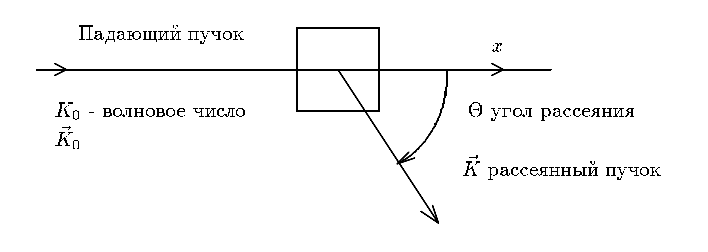
\includegraphics[scale=0.9]{Ris/ris_eps/ris4_1_01.eps}}}

\risp{1.1}{Опыт по дифракции}
\end{figure}

Если в случае дифракции пучков электронов и рентгеновских лучей
мы получаем мгновенную картину расположения частиц, то
из экспериментов по дифракции нейтронов мы получаем также сведения о
динамике отдельных частиц: $\lambda=(2\div5)$\hbox{\hbox{A}\hskip -2,08 mm \raise 1,5 mm\hbox{$^\circ$}}
сравнимо с $a$. Речь идет о холодных (тепловых) и ультра
холодных нейтронах.
\subzagl{Дифракция электромагнитного излучения в оптическом
диапазоне частот --- рассеяние света}

\markright{\hfill\small Дифракция электромагнитного излучения\hfill}

$\lambda=5\cdot10^{-5}$см; ${v}=c=3\cdot10^{10}\rm {см\over
сек}$, т.\ е. $\lambda\gg a$; $\Delta t\ll\tau$; однако высокая
точность экспериментов по рассеянию позволяет наблюдать
доплеровские смещения и уширения спектральных линий $\Delta\omega$, вызванные
тепловым движением молекул
$${\Delta \omega\over \omega}\approx{{v}_T\over
c}\simeq10^{-5}\div10^{-6}.$$
\noindent
Это позволяет получать информацию о молекулярной динамике.
Высокая точность оптического эксперимента по рассеянию света
стала возможна с появлением лазеров, спектроскопии высокой
разрешающей силы, регистрации сигнала в режиме счета фотонов.

Рассеянием света называется его распространение по
направлениям, отличным от направлений, предписываемых
макроскопическими уравнениями Максвелла.
В однородной среде свет распространяется по направлению преломленного и
отраженного луча, --- это результат интерференции вторичных
волн, излучаемых молекулярными электронами, возбужденными
световой волной. В однородной среде одинаковые элементы объема
содержат одинаковое число молекул, вторичные волны когерентны,
интерферируют и гасят друг друга по всем направлениям кроме
преломленного луча в среде.

В работе Л.~И. Мандельштам привел наглядное объяснение того факта,
что однородная среда свет не рассеивает. Пусть $V_1^*$ и $V_2^*$
--- физически малые объемы на расстоянии $l$ друг от друга таком,
что разность хода двух рассеянных лучей будет ${\lambda\over2}$.
${V}^*\ll\lambda^3$ содержат одинаковое число молекул.
Суммируя амплитуды в случае когерентных источников от ${
V}_1^*$ и ${V}_2^*$, если разность хода двух лучей
${\lambda\over2}$, получим в результате интерференции ноль. Для
каждого ${V}^*$ на конечном расстоянии $l$ можно найти такой
же физически малый объем при любом $\Theta$, кроме
$\Theta=0$
$$l={\lambda\over2\sin\Theta};$$
Для $\Theta=0$ не найдется конечного $l$ между ${V}_1^*$ и ${
V}_2^*$, чтобы разность хода была ${\lambda\over2}$.

Итак, причиной рассеянного света должны быть неоднородности:
\vskip 2mm
I. \ \ Мутная среда, частицы $d\geq\lambda$, эмульсии,
суспензии, аэрозоли; $n_{\rm частицы}\not=n_{\rm среды}$.
\vskip 2mm
II. \ Коллоидные растворы $d\geq\lambda$, но
$n_{\rm частицы}=n_{\rm среды}$.
\vskip 2mm
III. \hskip -0,4mm Молекулярное рассеяние света в <<оптически
пустой>>\ среде: жидкости, газы, состоящие\par
\ \ \ \ \ из одного\ \ сорта молекул. Неоднородности: \ флуктуации термодинамических величин:
\par \ \ \ \ \ $\Delta{\cal E},\ \Delta p,\ \Delta T,\ \Delta S$.

Причиной оптических неоднородностей
становятся флуктуации оптической диэлектрической проницаемости,
вызванные в свою очередь флуктуациями плотности вещества и
флуктуациями ориентации молекул. В однородных растворах
существенной дополнительной причиной молекулярного рассеяния
света становятся флуктуации концентрации компонентов раствора.
Каждое физическое явление, ведущее к возникновению рассеянного
света, накладывает свой характерный <<отпечаток>>\ на
интенсивность, поляризацию и спектральный состав рассеянного
света. Тем самым, изменения этих характеристик рассеянного света
позволяют изучать сами эти явления. При помощи рассеянного света
изучается структура молекул, определяются молекулярные веса
биологически активных молекул, размеры ионов, определяется число
Авогадро, исследуется кинетика флуктуаций и распространение
гиперзвука в конденсированных средах. С появлением лазеров в
настоящее время огромную роль в создании теории жидкого состояния
вещества играют исследования межмолекулярного взаимодействия и
молекул в жидкости по интегральной интенсивности и спектрам
рассеянного света.

\begin{figure}[tbp]
\centerline{\hbox{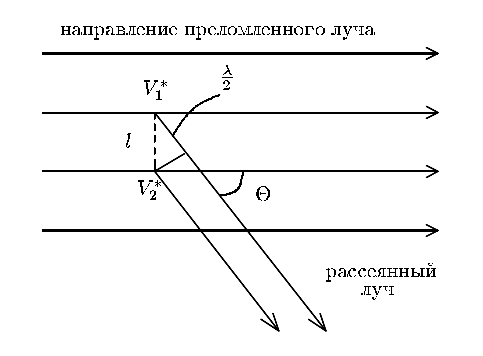
\includegraphics[scale=0.9]{Ris/ris_eps/ris4_1_02.eps}}}

\risp{1.2}{
Рассеяние в однородной
среде}
\end{figure}
\subzag{Теория Релея}
Первая теория молекулярного рассеяния света связана с именем
Релея. Рассмотрим рассеяние света на одной изолированной
молекуле. Пусть на молекулу падает монохроматическая световая
волна с циклической частотой $\omega$ и напряженностью
электрического поля $\vec E$
$$\vec E=\vec E_0\cos\omega t,\noq$$
где $\vec E_0$ --- амплитуда
поля. Мы начинаем рассмотрение с рассеяния линейно поляризованной
волны, так как в этом случае направление электрического поля
падающей волны точно фиксировано. Под действием переменного поля
в молекуле индуцируется переменный дипольный момент, величина
которого
$$\vec p=\alpha
\vec E=\alpha \vec E_0\cos\omega t,\eqno (1.4a)$$
где $\alpha$ --- поляризуемость
молекулы, который согласно электромагнитной теории сам излучает
электромагнитные волны.
Вектор напряженности поля излучения дается следующим
выражением:
$$\vec e=-{\omega^2\over c^2r^3}\vec r\times(\vec r\times\vec
p),\noq$$
где $c$ --- скорость света; $\vec r$ --- радиус-вектор, имеющий
направление от рассеивающей частицы в точку наблюдения; $\vec p$
--- вектор дипольного момента. Двойное векторное произведение
равно
$$\vec r\times(\vec r\times\vec p)=pr^2\sin\Phi,\noq$$
поэтому для численной величины вектора $\vec e$ получаем:
$$e={\omega^2\over c^2r}\alpha E\sin\Phi,\noq$$
где $\Phi$ --- угол между направлением напряженности
электрического поля падающей волны $\vec E$ и радиусом-вектором
$\vec r$.

Интенсивность света пропорциональна среднему от квадрата
напряженности электрического поля. При соответствующем выборе
единиц измерения можно положить коэффициент пропорциональности
равным единице и тогда будем иметь для интенсивности падающего и
рассеянного света:
$$I_0=E_0^2\overline{\cos^2\omega t},\hskip 4mm
i=I_0{\omega^4\over c^4r^2}\alpha^2\sin^2\Phi,\noq$$
или, заменив $\omega$ на $\omega={2\pi
c\over\lambda}$, где $\lambda$ --- длина световой волны, получаем
$$i=I_0{16\pi^4\over\lambda^4r^2}\alpha^2\sin^2\Phi.\noq$$
Релей считал, что из-за теплового движения молекул источники
некогерентны и можно складывать интенсивности, тогда
$$I=I_0{16\pi^4\over\lambda^4r^2}N_0V\alpha^2\sin^2\Phi,\noq$$
где $N=N_0V$, $N_0$ --- число молекул в 1 $\rm см^{3}$. Для газов
можно положить $\alpha={n-1\over2\pi N_0}$, тогда интенсивность
рассеянного света равна
$$I=I_0{2\pi^2\over\lambda^4r^2}{(n-1)^2V\over
N_0}\sin^2\Phi.\noq$$
\subzag{Теория Эйнштейна-Смолуховского}
Однородное распределение молекул удовлетворяет II началу
термодинамики, --- максимум энтропии системы. II начало ---
статистическая закономерность, т. е. возможно отклонение
состояния системы от ее наиболее вероятного состояния. Эти
отклонения характеризуются малыми величинами --- {\it
флуктуациями} термодинамических величин:
$$\Delta\rho=\rho-\bar\rho;\hskip 4mm\Delta n=n-\bar n;\hskip
4mm\Delta{\cal E}={\cal E}-\bar{\cal E};\hskip 4mm \Delta
p=p-\bar p\ \hbox{и т. п.}$$

В 1907 году Л.И. Мандельштам показал, что объяснение Рэлеем
некогерентности источников тепловым движением справедливо, когда
молекул мало, в случае большого объема содержащего много молекул
роль источников играют физически малые объемы.
Физически малый объем $v^*$ --- объем, линейные размеры
которого малы, по сравнению с длиной волны света, т. е.
$V^*\ll\lambda^3$,  но в нем содержится достаточно много молекул,
чтобы можно было производить статистические расчеты. Флуктуации
плотности (числа частиц) в физически малом объеме определяют
флуктуации оптической диэлектрической проницаемости, которые и
являются причиной, вызывающей оптическую неоднородность среды,
что приводит к возникновению рассеяния света в оптически <<пустых>>\ средах.
Плодотворная идея Смолуховского (1908 г.) о флуктуациях
плотности, как о причине рассеяния света легла в основу
статистической теории рассеяния света, развитой Эйнштейном в 1910
г.

Разобьем рассеивающий объем на физически малые объемы ${v}^*$; напряженность,
создаваемая диполями в физически малых объемах
$$e_{v^*}=eN=-{\omega^2\over e^2r}N\alpha E\sin\Phi.\noq$$
Однородному распределению соответствует $\bar N$:
$$\bar e_{v^*}=-{\omega^2\over c^2r}\bar N\alpha E\sin\Phi.\noq$$
Так как $N=\bar N+\Delta N$, то:
$$\Delta e_{v^*}=-{\omega^2\over c^2r}\Delta N\alpha E\sin\Phi.\noq$$
Интенсивность света, рассеянного физически малым объемом:
$$i_{v^*}=\overline{\Delta e_{v^*}^2}=I_0{\omega^4\over
c^4r^2}\overline{(\Delta N)^2}\alpha^2\sin^2\Phi.\noq$$
Статистическая физика показывает, что в отсутствие взаимодействия
для идеального газа
$\overline{(\Delta N)^2}=\bar N=N_0{v^*}$, тогда
$$i_{v^*}=I_0{16\pi^4\over
\lambda^4r^2}N_0{v^*}\alpha^2\sin^2\Phi.\noq$$
Флуктуации числа частиц независимы в разных физически малых
объемах, поэтому
$$I=I_0{16\pi^4\over\lambda^4r^2}N_0V\alpha^2\sin^2\Phi.\noq$$
Это та же формула, что и у Рэлея.

Рассмотрим геометрию эксперимента по рассеянию света. Пусть
верхний индекс обозначает поляризацию вектора $\vec E$ падающего
луча, а нижний --- поляризацию рассеянного света. Падающий луч
распространяется вдоль оси $x$.

\begin{figure}[tbp]
\centerline{\hbox{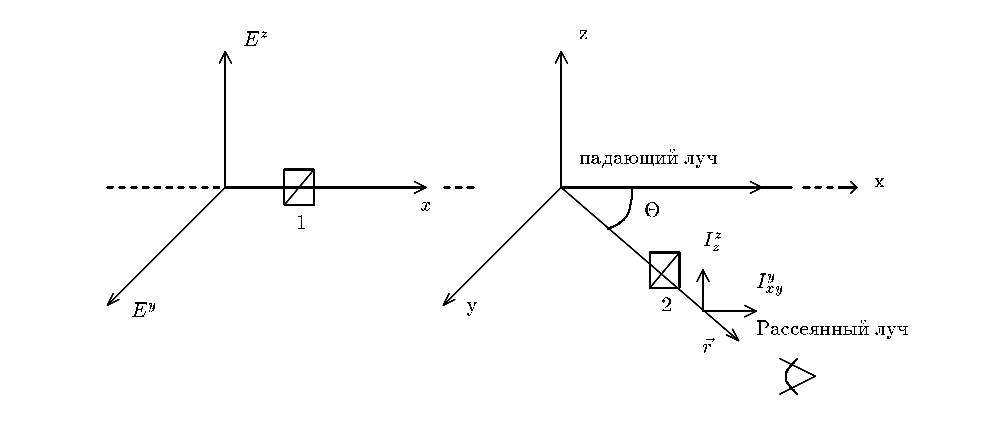
\includegraphics[scale=0.9]{Ris/ris_eps/ris4_1_03.eps}}}

\risp{1.3}{
Геометрия эксперимента по рассеиванию
света}
\end{figure}



Поворотом поляризационной призмы 1 мы можем менять поляризацию
падающего луча, а поворотом призмы 2 выделять из рассеянного
света компоненты с нужной поляризацией.
\par I. \ Падающий луч поляризован по оси $z$. $\Phi$ --- угол между
радиусом вектором в плоскости $xy$ и $E^z$ равен $\pi\over2$:
$$I_{z}^{z}=I_0{16\pi^4\over\lambda^4r^2}N_0V\alpha^2.\noq$$
\par II. Падающий луч поляризован по оси $y$:
$$\Phi={\pi\over2}-\Theta;\hskip 4mm\sin^2\Phi=\cos^2\Theta,$$
$$I_{xy}^y=I_0{16\pi^4\over\lambda^4r^2}N_0V\alpha^2\cos^2\Theta.\noq$$
Индикатриса рассеяния имеет следующий вид (рис. 4.1.4):\par

\begin{figure}[tbp]
\centerline{\hbox{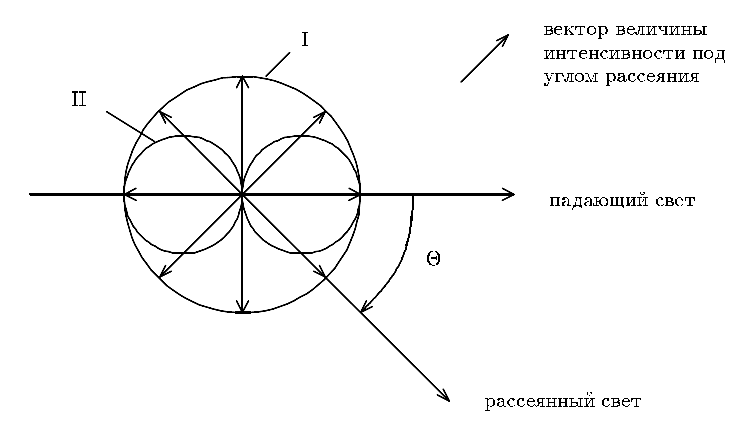
\includegraphics[scale=0.9]{Ris/ris_eps/ris4_1_04.eps}}}

\risp{1.4}{
Индикатриса рассеяния}
\end{figure}

III. Если падает естественный свет ${I_0\over2}$ ---
интенсивность отдельных поляризованных компонентов, то полная
интенсивность
$$I=I_0{8\pi^4\over\lambda^4r^2}N_0V\alpha^2(1+\cos^2\Theta).\noq$$
Для газов уравнение Лорентц-Лоренца
$$2\pi N_0\alpha=n-1;\hskip 4mm \alpha={n-1\over 2\pi N_0},$$
тогда
$$I=I_0{2\pi^2\over\lambda^4r^2}(n-1)^2{V\over
N_0}(1+\cos^2\Theta).\noq$$
Итак, видно из формулы:

1) $I\sim{1\over\lambda^4}$;

2) индикатриса рассеяния симметрична относительно плоскости,
перпендикулярной падающему лучу (рассеяние <<вперед>>\ и <<
назад>>\ одинаково);

3) свет, рассеянный под углом $90^{\circ}$ полностью
поляризован. 

На пути рассеянного луча ставят поляризационную призму
и ее поворотом выделяют $I_{xy}$ и $I_z$. Величину $\Delta$
называют степенью поляризации и определяют выражением
$$\Delta={I_{xy}\over I_{z}}=\cos^2\Theta;\hskip 4mm \hbox{Если}\
\Theta=90^{\circ}\hbox{, то\ }{I_x\over I_z}=0,\ \Delta=0,$$

\begin{figure}[tbp]
\centerline{\hbox{\includegraphics[scale=0.9]{Ris/ris_eps/ris4_1_05.eps}}}

\risp{1.5}{
Поляризация рассеянного света}
\end{figure}


На опыте оказывается, что $\Delta>0$; Для газов $\Delta<0,1$. Это
означает, что молекулы поляризуются анизотропно, т. е. при $I^z$
поляризации появляется помимо $I_{z}^z$ компонента $I_x^z$ в
плоскости рассеяния $xy$ (см. рис. 4.1.5).\par
\subzag{Деполяризованное рассеяние света в газах}
Молекулы поляризуются анизотропно, $\Delta\not=0$. К рассеянию на
флуктуациях плотности необходимо прибавить рассеяние на
флуктуациях ориентации анизотропных молекул. Если молекулы
поляризуются анизотропно, то направление индуцированного
дипольного момента не совпадает с направлением поля $\vec E$,
падающего на образец.

Составляющие дипольного момента в лабораторной системе координат
$x,\ y,\ z$:
$$p_i=\sum\limits_{k=x,y,z}\alpha_{ik}E_k.$$

\begin{figure}[tbp]
\centerline{\hbox{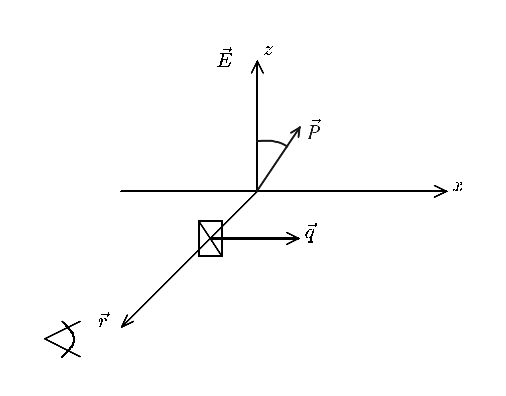
\includegraphics[scale=0.9]{Ris/ris_eps/ris4_1_06.eps}}}

\risp{1.6}{
Дипольный момент молекулы}
\end{figure}

Различные молекулы представляют диполи с любой ориентацией, все
ориентации равновероятны. Поля излучений диполей спроектируем на
вектор $\vec q$, лежащий в плоскости главного сечения
поляризационной призмы, причем $\vec q\perp\vec r$.
$$e_{q}=\vec e\cdot\vec q=-{\omega^2\over c^2r^3}(\vec
r\times(\vec r\times\vec p))\cdot\vec q.\noq$$
Используя формулу представления двойного векторного произведения
\begin{plain}
$$\eqalign{e_q=&-{\omega^2\over c^2r^3}\left\{\left[\vec r(\vec r\cdot\vec
p)-\vec p(\vec r\cdot\vec r)\right]\cdot\vec q\right\},\cr
e_q=&-{\omega^2\over c^2r^3}\left\{(\vec r\cdot\vec
q)(\vec r\cdot\vec p)-r^2(\vec p\cdot\vec q)\right\}.}$$
\end{plain}
Так как $\vec q\perp\vec r$, то $(\vec r\cdot\vec q)=0$, и
$$e_q={\omega^2\over c^2r}(\vec p\cdot\vec q),\hskip 4mm
i_q={\omega^4\over c^4r^2}\overline{(\vec p\cdot\vec q)^2},\noq$$
где $\overline{(\vec p\cdot\vec q)^2}$ --- среднее по всем
ориентациям молекул. Подобно тому, как мы суммировали
интенсивности рассеяния от отдельных изотропных молекул,
содержащихся в объеме рассеяния, поступим также, считая, что
анизотропные молекулы газа рассеивают свет независимо друг от
друга. Попутно произведем замену $\omega$ на
$2\pi{c\over\lambda}$ и умножим на число молекул в рассеивающем
объеме $N_0\cdot V$.
$$I_q={16\pi^4\over\lambda^4r^2}\overline{(\vec p\cdot\vec
q)^2}N_0V.\noq$$
Вычислим $\overline{(\vec p\cdot\vec q)^2}$. Рассчитаем сначала
скалярное произведение векторов $\vec p$ и $\vec q$. С этой
целью проведем две системы координат: неподвижную в пространстве
(лабораторную) систему $x$, $y$, $z$ и молекулярную {\it 1, 2,
3,} связанную с выбранной молекулой и проведенной по главным осям
тензора поляризуемости молекулы. Первую систему проведем
следующим образом: ось $z$ направляем вдоль вектора $\vec E$
электрического поля падающей волны. Затем из начала координат
проводим единичный вектор поляризации $\vec q$ (рис. 4.1.7). После
этого проведем ось  $x$ так, чтобы она лежала в плоскости оси
$z$ и вектора $\vec q$. Ось $y$ можно не проводить. Направления
падающего луча мы не указываем. Нужно помнить, что падающий луч
перпендикулярен оси $z$. Рассеянный луч перпендикулярен вектору
$\vec q$.

\begin{figure}[tbp]
\centerline{\hbox{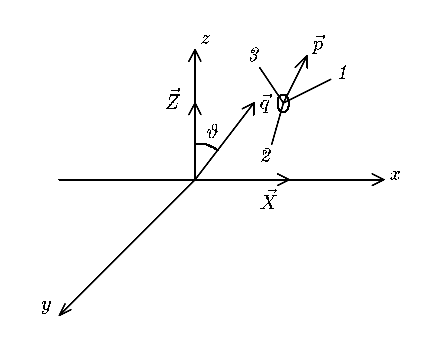
\includegraphics[scale=0.9]{Ris/ris_eps/ris4_1_07.eps}}}

\risp{1.7}{
Лабораторная и молекулярная системы
координат}
\end{figure}


Проведем в лабораторной системе координат еще два единичных
вектора: вектор $\vec X$ вдоль оси $x$ и вектор $\vec Z$ вдоль оси
$z$. Таким образом, все три единичных вектора лежат в одной
плоскости. Выразим единичный вектор $q$ через $\vec X$ и $\vec
Z$. С этой целью спроектируем вектор $\vec q$ на оси $x$ и $z$.
Проекции равны $q\sin\theta$ и $q\cos\theta$. Но так как
$q=1$, то проекции равны просто $\sin\theta$ и
$\cos\theta$. Умножив первую величину на единичный вектор
$\vec X$ и вторую на $\vec Z$, мы можем изобразить вектор $\vec
q$ в виде геометрической суммы двух векторов
$$\vec q=s\vec X+c\vec Z, \noq$$
где $s=q\sin\theta$, $c=q\cos\theta$.
Проведем расчет скалярного произведения $(\vec p\cdot\vec q)$
в молекулярной системе координат $\sigma\ ({\it 1,2,3})$:
$$(\vec p\cdot\vec q)=\sum\limits_{\sigma}p_{\sigma}q_{\sigma}
\noq$$
Воспользуемся для этой цели единичными векторами $\vec X$ и $\vec
Z$. Прежде всего выразим напряженность электрического поля
падающей волы $\vec E$ через произведение длины вектора $E$ на
единичный вектор $\vec Z$: $\vec E=E\vec Z$. Тогда для проекции
вектора $\vec p$ на оси {\it 1, 2, 3} будем иметь
$$ p_i=\sum\limits_{k=x,y,z}\alpha_{ik}E_k; \noq$$
$$ p_i=\sum\limits_{\sigma}p_{\sigma}(\sigma i); \eqno (1.27а)$$
$$ E_{\sigma}=\sum\limits_i E_i(\sigma i); \eqno(1.27б) $$
$$p_{\sigma}=\alpha_{\sigma}E_{\sigma}=E\alpha_{\sigma}Z_{\sigma}. \eqno
(1.27в)$$
Из \eqn{26}, \eqn{25} и \eqn{27$в$} получаем
$$ (\vec p\cdot\vec
q)=E\sum\limits_{\sigma=1,2,3}\alpha_{\sigma}Z_{\sigma}(sX_{\sigma}+cZ_{\sigma})
.\noq$$
Проекции единичных векторов на оси ({\it 1, 2, 3})
$X_{\sigma}$ и $Z_{\sigma}$ являются направляющими косинусами
$X_{\sigma}=\cos(x,\sigma)$,
$Z_{\sigma}=\cos(z,\sigma)$. Возведя в квадрат \eqn{28},
получим сумму трех слагаемых:
$$(\vec p\cdot\vec
q)=E^2\left\{\sum\limits_{\sigma}\alpha_{\sigma}^2Z_{\sigma}^2(sX_{\sigma}+cZ_{\sigma})^2
+\right.$$ $$\left.+2\sum\limits_{\sigma}\sum\limits_{\Omega}\alpha_{\sigma}\alpha_{\Omega}\cdot
Z_{\sigma}Z_{\Omega}(sX_{\sigma}+cZ_{\sigma})(sX_{\Omega}+cZ_{\Omega})\right\},
\eqno (1.28а)$$
где $\sigma=${\it 1, 2, 3} и $\Omega=${\it 1, 2, 3}.
При переходе к усреднению следует обратить внимание на то, что
оси {\it 1, 2, 3} принимают все возможные направления и тем
самым становятся равноправными, откуда следуют следующие
равенства:
$$Z_1^2(sX_1+cZ_1)^2=Z_2^2(sX_2+cZ_2)^2=$$ $$Z_3^2(sX_3+cZ_3)^2,
Z_1Z_2(sX_1+cZ_1)(sX_2+cZ_2)=$$ $$Z_1Z_3(sX_1+cZ_1)(sX_3+cZ_3)=$$ $$=
Z_2Z_3(sX_2+cZ_2)(sX_3+cZ_3).\eqno (4.28б)$$
$$\overline{(\vec p\cdot\vec
q)^2}=\vec E^2\left\{(\alpha^2_1+\alpha^2_2+\alpha^2_3)\overline{z^2_1(sx_1+cz_1)^2}+
2(\alpha_1\alpha_2+\alpha_1\alpha_3+\alpha_2\alpha_3)\cdot$$ $$\cdot z_1z_2(sx_1+cz_1)
(sx_2+cz_2)\right\}$$
Обозначим
$$\alpha_1^2+\alpha_2^2+\alpha_3^2\equiv A,$$
$$\alpha_1\alpha_2+\alpha_1\alpha_3+\alpha_2\alpha_3\equiv
B,\noq$$
Выражение для $\overline{(\vec p\cdot\vec q)^2}$ принимает вид:
$$\overline{(\vec p\cdot\vec
q)^2}=\overline{E^2}\left\{A\overline{Z_1^2(sX_1+cZ_1)^2}+2B\overline{Z_1Z_2(
sX_1+cZ_1)(sX_2+cZ_2)}\right\},\noq$$
и раскрыв скобки, получаем:
$$\overline{(\vec p\cdot\vec
q)^2}=\overline{E^2}\left\{A\left[\overline{Z_1^2s^2X_1^2}+\overline{c^2
Z_1^4}+2s\overline{cX_1Z_1^3}\right]+\right.$$
$$\left.+B\left[\overline{s^2X_1 X_2
Z_1Z_2}+\overline{c^2Z_1^2Z_2^2}+s\overline{cX_1Z_1Z_2^2}+sc\overline{X_2Z_2Z_1^2}\right]\right\}.\eqno
(1.30а)$$

Здесь $X_1$, $X_2$, $Z_1$, $Z_2$ представляют собой, как
отмечалось выше, направляющие косинусы
между осями  $x$, $z$, и {\it 1,2} соответственно, поэтому
задача сводится к вычислению средних значений от произведений
косинусов [см. Глава 1, стр. 12]. Известно,
что
\begin{plain}
$$\eqalign{\overline{X_1Z_1^3}=\overline{X_1Z_1Z_2^2}=&\overline{X_2Z_1^2Z_2}=0,\cr
\overline{Z_1^4}={1\over5};\hskip 4mm
\overline{X_1^2Z_1^2}=&{1\over15};\hskip 4mm\overline{X_1Z_1
Z_2X_2}=-{1\over30}.}\noq$$
\end{plain}
Предварительно, для того, чтобы произвести
разделение излучения на рассеяние от флуктуаций плотности и от
флуктуаций анизотропии, введем вместо сокращенных обозначений $A$
и $B$ величины $\alpha$ и $\gamma^2$, имеющие более ясный
физический смысл:$\alpha$ --- средняя поляризуемость и $\gamma^2$
--- оптическая анизотропия молекул:
\begin{plain}
$$\eqalign{
\alpha={1\over3}&(\alpha_1+\alpha_2+\alpha_3),\cr
\gamma^2={1\over2}\left\{(\alpha_1-\alpha_2)^2\right.&\left.+(\alpha_1-\alpha_3)^2+
(\alpha_2-\alpha_3)^2\right\}.}\noq$$
\end{plain}
Подставим \eqn{31} в \eqn{30}, заменив $s^2=1-c^2$,
$c^2=\cos^2\theta$. Согласно \eqn{29}
$$A=3\alpha^2+{2\over3}\gamma^2;\hskip 4mm
B=6\alpha^2-{2\over3}\gamma^2;$$
$$\overline{(\vec p\cdot\vec
q)^2}=\overline{E^2}\left\{(\alpha^2+{1\over45}\gamma^2)\cos^2\theta
+{3\over45}\gamma^2\right\}.\noq$$
Мы вычислили среднюю величину $\overline{(\vec p\cdot\vec q)^2}$,
которая входит в выражение \eqn{24} для интенсивности рассеяния
света от газа с анизотропными молекулами. Подставив
в выражение для $I_q$ и заменив одновременно $\overline{E^2}$ на
$I_0$, получаем:
$$I_q=I_0{16\pi^4\over\lambda^4r^2}N_0V\left\{\alpha^2\cos^2\theta+\gamma^2
\left({3\over45}+{1\over45}\cos^2\theta\right)\right\}.\noq$$
Таким образом, мы представили полную интенсивность светорассеяния
газа в виде суммы двух слагаемых: рассеяния от флуктуации
плотности, которое пропорционально $\alpha^2$, и рассеяния от
флуктуации анизотропии которое пропорционально $\gamma^2$. Можно
показать, что первое слагаемое в формуле \eqn{34} тождественно с
выражением \eqn{17} для интенсивности рассеяния изотропными
молекулами газа, если там на пути рассеянного луча поставить
поляризационную призму. В самом деле, если луч пройдет через
поляризационную призму, то в выражении \eqn{17} для интенсивности
вместо $\sin^2\Phi$ будет стоять $\sin^2\Phi\cos^2\psi$, где
$\psi$ --- угол между векторами $\vec e$ и $\vec q$, и тогда это
выражение будет тождественно с первым слагаемым формулы \eqn{34},
так как можно доказать, что $\sin\Phi\cos\psi=\cos\theta$. В
дальнейшем для краткости мы часто будем называть рассеяние света
на флуктуациях плотности изотропным рассеянием, а рассеяние света
на флуктуациях ориентации --- анизотропным или деполяризованным
рассеянием света.

Обычно изучают рассеяние света под прямым углом. Проведем
координатные оси $x$, $y$, $z$ (см. рис. 4.1.8) и направим ось $x$
вдоль падающего луча, а ось $y$ --- по направлению рассеянного
луча. Рассмотрим рассеяние поляризованного света в двух случаях:
электрический вектор падающей волны направлен по оси $z$ и этот
же вектор направлен по оси $y$.

\begin{figure}[tbp]
\centerline{\hbox{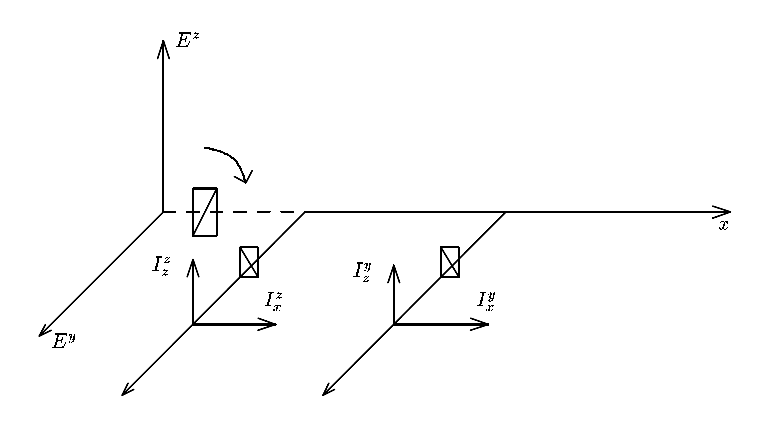
\includegraphics[scale=0.9]{Ris/ris_eps/ris4_1_08.eps}}}

\risp{1.8}{
Рассеяние под прямым
углом}
\end{figure}


I. Сначала рассмотрим случай, когда угол рассеяния $\Theta=90^{\circ}$.
\vskip 1mm
 {\it 1. Электрическое поле падающей волны направлено по оси $z$}.
\vskip 1mm
\noindent
Воспользуемся формулой \eqn{34}. Поместим на пути рассеянного
луча поляризационную призму и повернем ее так, чтобы в одном
случае вектор поляризации $\vec q$ был направлен по оси $x$, а во
втором случае по оси $z$. Обозначим соответствующие интенсивности
рассеянных лучей через $I_x^z$ и $I_z^z$. Для $x$-компоненты
рассеянного луча $\theta={\pi\over2}$, $\cos\theta=0$ и
поэтому формула \eqn{34} дает
$$I_x^z=I_0{16\pi^4\over\lambda^4r^2}N_0V{3\over45}\gamma^2.\noq$$
Для $z$-компоненты $\theta=0$, $\cos\theta=1$ и поэтому
$$I_z^z=I_0{16\pi^4\over\lambda^4r^2}N_0V(\alpha^2+{4\over45}\gamma^2).\noq$$
Полная интенсивность равна сумме
$$I^z=I_0{16\pi^4\over\lambda^4r^2}N_0V(\alpha^2+{7\over45}\gamma^2).\noq$$

{\it 2. Электрическое поле падающей волны направлено по оси
$y$.}
\vskip 1mm
\noindent
Ориентируем поляризационную призму по-прежнему так, чтобы сначала
вектор поляризации $\vec q$ был направлен по оси $x$, а потом по
оси $z$. Здесь в обоих случаях $\theta=90^{\circ}$,
$\cos\theta=0$ и поэтому для соответствующих компонент будем
иметь
$$I_x^y=I_z^y=I_0{16\pi^4\over\lambda^4r^2}N_0V{3\over45}\gamma^2,\noq$$
отсюда для полной интенсивности получаем
$$I^y=I_0{16\pi^4\over\lambda^4r^2}N_0V{6\over45}\gamma^2.\noq$$

\par
{\it 3. Электрическое поле падающей волны неполяризовано.}
Воспользуемся для этой цели уже известным нам приемом ---
мысленным разложением естественного падающего света на два
поляризованных луча: на луч с электрическим вектором,
направленным по оси $z$, и на луч с электрическим вектором по оси
$y$. Рассеяние от каждого поляризованного луча описывается
формулами \eqn{35} и \eqn{38}. Здесь тоже на пути рассеянного
луча ставим поляризационную призму. Обозначим через $I_x$
интенсивность рассеяния, когда вектор поляризации $\vec q$
направлен по оси $x$, и через $I_z$ --- когда вектор поляризации
направлен по оси $z$. Нетрудно видеть, что
$$I_x^z=I_z^z={I^z\over2};\hskip 4mm
I_x^y=I_z^y={I^y\over2},$$
$$I_x=I_x^z+I_x^y;\hskip 5mm I_z=I_z^z+I_z^y,$$
и сложив получаем
$$I_x=I_0{8\pi^4\over\lambda^4r^2}N_0V{6\over45}\gamma^2,\noq$$
$$I_z=I_0{8\pi^4\over\lambda^4r^2}N_0V(\alpha^2+{7\over45}\gamma^2).\noq$$
Полная интенсивность рассеяния света под углом $\Theta=90^{\circ}$
будет равна сумме $I_x$ и $I_y$:
$$I=I_0{8\pi^4\over\lambda^4r^2}N_0V\left(\alpha^2+{13\over45}\gamma^2\right).\noq$$

II. Теперь рассмотрим случай $\Theta\not=90^{\circ}$. Поступим таким
же образом, как и раньше, --- разложим мысленно падающий свет на
два поляризованных луча с электрическим вектором по осям $z$ и
$y$. Рассеянный луч также разложим на два поляризованных луча ---
на луч с электрическим вектором параллельно плоскости рассеяния,
т. е. в плоскости $xy$, и на луч с электрическим вектором
перпендикулярно этой плоскости, или иначе говоря, параллельно оси
$z$.

\begin{figure}[tbp]
\centerline{\hbox{\includegraphics[scale=0.9]{Ris/ris_eps/ris4_1_09.eps}}}

\risp{1.9}{
К расчету интенсивности
рассеянного света при углах рассеяния $\Theta\not=90^{\circ}$}
\end{figure}

Компоненты $I_{xy}^z,\ I_z^z,\ I_{xy}^y,\ I_z^y$ рассеянного
излучения выделяются поворотом поляризационной призмы при двух
поляризациях падающего света.
Согласно \eqn{34}:
$$I_q=I_0{16\pi^4\over\lambda^4r^2}\left\{\alpha^2\cos^2\theta
+\gamma^2\left({3\over4}+{1\over45}\cos^2\theta\right)\right\},$$
и так как $\theta=\Theta$, то
$$I_{xy}^z=I_0{16\pi^4\over\lambda^4r^2}N_0V{3\over45}\gamma^2,\noq$$
$$I_z^z=I_0{16\pi^4\over\lambda^4r^2}N_0V\left\{\alpha^2+{4\over45}\gamma^2\right\},\noq$$
$$I_z^y=I_0{16\pi^4\over\lambda^4r^2}N_0V{3\over45}\gamma^2,\noq$$
$$I_{xy}^y=I_0{16\pi^4\over\lambda^4r^2}N_0V\left\{\alpha^2\cos^2\Theta+\gamma^2
\left({3\over45}+{1\over45}\cos^2\Theta\right)\right\}.\noq$$
Сравним $I_{xy}^y$ с $I_x^y$ для случая $\Theta=90^{\circ}$:
$$I_x^y=I_0{16\pi^4\over\lambda^4r^2}N_0V{3\over45}\gamma^2.$$
Для естественного падающего света формула для интенсивности
рассеяния под углом $\Theta$ имеет вид:
$$I_{\Theta}=I_0{8\pi^4\over\lambda^4r^2}N_0V\left\{\alpha^2(1+\cos^2\Theta)+
\gamma^2\left({13\over45}+{1\over45}\cos^2\Theta\right)\right\}.\noq$$
\subzag{Степень деполяризации рассеянного света}
Будем рассматривать рассеяние под прямым углом к падающему лучу.
Во всех предыдущих вычислениях мы раскладывали рассеянный луч на
две поляризованные составляющие $I_x$ и $I_y$, в которых
электрический вектор направлен соответственно по оси $x$ или
параллельно падающему лучу, и по оси $z$ --- перпендикулярно
падающему лучу. Отношение интенсивности первой составляющей ко
второй, как мы уже знаем из предыдущего, называется коэффициентом
или степенью деполяризации.

В случае, когда падающий луч поляризован так, что его
электрический вектор направлен по оси $z$, а наблюдение
рассеянного луча происходит по оси $y$, коэффициент деполяризации
обозначают обычно через $\Delta_v$. Из формул \eqn{35} и \eqn{36}
находим, что
$$\Delta_v={I_x^z\over
I_z^z}={{3\over45}\gamma^2\over\alpha^2+{4\over45}\gamma^2}.\noq
$$

В другом случае, когда электрический вектор в падающем луче
направлен по оси $y$ (горизонтально), совпадающим с направлением
наблюдения рассеянного луча, коэффициент деполяризации обозначают
через $\Delta_h$. Согласно формуле \eqn{38}
$$\Delta_h={I_x^y\over I_z^y}=1.\noq$$

Наконец, когда падающий луч неполяризован, из формул \eqn{40} и
\eqn{41} находим
$$\Delta={I_x\over
I_z}={{6\over45}\gamma^2\over\alpha^2+{7\over45}\gamma^2}.\noq$$
Если молекулы изотропны, то $\gamma^2=0$ и $\Delta_v=0$,
$\Delta=0$. Чтобы найти связь между двумя коэффициентами
деполяризации $\Delta_v$ и $\Delta$, умножим \eqn{48} на 2 и
разделим на \eqn{50}
$${2\Delta_v\over\Delta}={\alpha^2+{7\over45}\gamma^2\over\alpha^2+{4\over45}
\gamma^2}=1+\Delta_v,$$
откуда получаем
$$\Delta={2\Delta_v\over1+\Delta_v}.\noq$$
Все наши формулы начиная с \eqn{34} изображают полную
интенсивность светорассеяния в виде суммы изотропного и
анизотропного рассеяний. Поэтому мы можем рассчитать по
отдельности коэффициенты деполяризации изотропного и
анизотропного рассеяний света. У изотропного рассеяния, как мы
знаем, оба коэффициента деполяризации равны нулю. Коэффициенты
деполяризации анизотропного рассеяния можно рассчитать с помощью
формул \eqn{35}, \eqn{40}, \eqn{41}. Нетрудно видеть, что для
анизотропного рассеяния $\Delta_v={3\over4}$, $\Delta={6\over7}$.
Из формул \eqn{48} и \eqn{50} следует, что коэффициенты
деполяризации рассеянного света $\Delta_v$ и $\Delta$
удовлетворяют следующим условиям:
$$\Delta_v\leq{3\over4},\hskip 4mm \Delta\leq{6\over7}.$$
Если заменить
$\alpha^2$ на ${(n-1)^2\over4\pi^2N_0^2}$, а $\gamma^2$ выразить
через $\Delta$:
$$\gamma^2=45\alpha^2{\Delta\over6-7\Delta},\noq$$
$$\gamma^2=45
\alpha^2{\Delta_v\over3-4\Delta_v},\noq$$
то полную интенсивность можно записать в виде:
$$I=I_0{2\pi^2\over\lambda^4r^2}{(n-1)^2\over N_0}\cdot V\times
{6+6\Delta\over6-7\Delta}\noq$$
Здесь первый множитель выражает рассеяние на флуктуациях
плотности, формула Рэлея-Энштейна. А второй множитель,
${6+6\Delta\over6-7\Delta}$ называют {\it фактором Кабанна} и
обозначают $f$. Если молекулы изотропны, то этот множитель равен
единице. В противном случае он больше единицы.

Можно измерять (вычислять) $I_{из}$ и умножать на $f$, чтобы
получить полное рассеяние. В современной литературе $I^z\equiv
I^v$; $I_z^z\equiv I_v^v$, индекс $v$ означает направление перпендикулярно плоскости
рассеяния (<<вертикально>>), $I_y\equiv I_h$; $I_{xy}\equiv I_h$;
$I_x^y\equiv I_h^v$. Индекс $h$ означает <<горизонтально>>, т. е.
параллельно плоскости рассеяния.
\subzag{Измерение степени деполяризации $\Delta$ рассеянного
света}
Измерение коэффициента деполяризации производится либо визуальным,
либо фотографическим, либо фотоэлектрическим методом. На рис.
4.1.10 представлена установка для визуального измерения степени
деполяризации. Параллельный пучок света от источника падает на
трубку Вуда. Рассеянный пучок, наблюдаемый под углом
$90^{\circ}$, проходит через поляризационную призму Волластона.
На выходе из призмы получаются два луча, поляризованные во
взаимно перпендикулярных плоскостях. Вращением николя добиваются,
чтобы два луча имели одинаковую яркость. Регистрирующим
устройством является кубик Люмера. Если $\Psi$ --- угол
между осью $x$ и главной плоскостью сечения николя, то
$$E_x\cos\Psi=E_z\sin\Psi;\hskip 4mm{E_x\over
E_z}=\hbox{tg}\Psi;\hskip 4mm \Delta={I_x\over
I_z}=\hbox{tg}^2\Psi.$$

\begin{figure}[tbp]
\centerline{\hbox{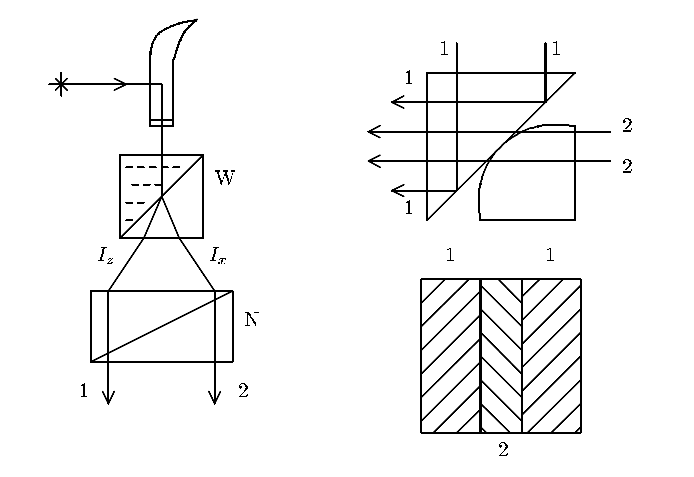
\includegraphics[scale=0.9]{Ris/ris_eps/ris4_1_10.eps}}}

\risp{1.10}{
Установка для
визуального метода измерения степени деполяризации}
\end{figure}

Найти $\Psi$ можно следующим способом. Вращением поляризатора
(николя) находят положение при котором яркости двух лучей равны,
затем находят второе такое же положение. Угол между этими
положениями будет $2\Psi$ или $180-2\Psi$. В кубике Люмера
сравниваются яркости двух полей, среднего (1) и бокового (2).

При фотоэлектрической регистрации на пути рассеянного луча ставится поляризационная призма
или поляроид. Рассеянный луч принимается фотоумножителем. При
вращении поляризатора вокруг оси фототок будет меняться в
некотором интервале. Минимальное значение фототока будет при
таком повороте поляризатора, когда его главная плоскость
параллельна оси $x$, и тогда получаем $x$-компоненту рассеянного
света, а максимальное --- при повороте на $90^{\circ}$, когда
главная плоскость параллельна оси $z$. Это дает $z$-компоненту
рассеянного света. Если сила фототока строго пропорциональна
освещенности, то отношение минимального фототока к максимальному
будет равно отношению интенсивностей этих двух составляющих
рассеянного света
$${I_{\rm min}^{\rm фототок}\over
I_{\rm max}^{\rm фототок}}=\Delta,$$
т. е. равно коэффициенту деполяризации. Так как
фотокатод не одинаково чувствителен к лучам различной
поляризации. Поэтому рекомендуется превратить линейно
поляризованный луч в циркулярно поляризованный перед направлением
на фотокатод, что можно осуществить с помощью пластинки в четверть
длины волны.

Измерение степени деполяризации требует применения надежных мер
во избежание возможных погрешностей. В особенности это относится
к газам и парам, у которых коэффициенты деполяризации очень малы
и само светорассеяние слабо.
Основными источниками ошибок являются пыль и паразитный свет.
Нестрогая геометрия опыта, неточная установка
поляризационных призм, а также двойное лучепреломление во
входном и выходном
окошках сосуда вследствие оставшихся там напряжений также могут
быть источниками погрешности.

Если за $\Delta'$ примем экспериментальное значение степени
деполяризации, а за $\Delta$ --- истинное ее значение, то
$$\Delta'={I_x+I_{\rm параз}\over I_z+I_{\rm параз}};\hskip 4mm
\Delta'>\Delta.$$
Интенсивность любого отраженного света в трубке
для рассеяния составляет величину
порядка $(0,1\div 0,001)I_0$, а, например, для жидкости
интенсивность самого рассеянного света $\sim
I_0\cdot 10^{-6}$.

Есть несколько способов избежать ошибок:

\noindent\hangindent 1cm\hangafter 4
1. в эксперименте использовать только трубку Вуда, а для
приготовления исследуемой жидкости использовать процедуру Мартина
и Лермана (см. рис. 4.1.11). Эта процедура состоит в тройном
замораживании, откачивании и последовательном ополаскивании
стеклянного шарика и трубки.

\begin{figure}[tbp]
\centerline{\hbox{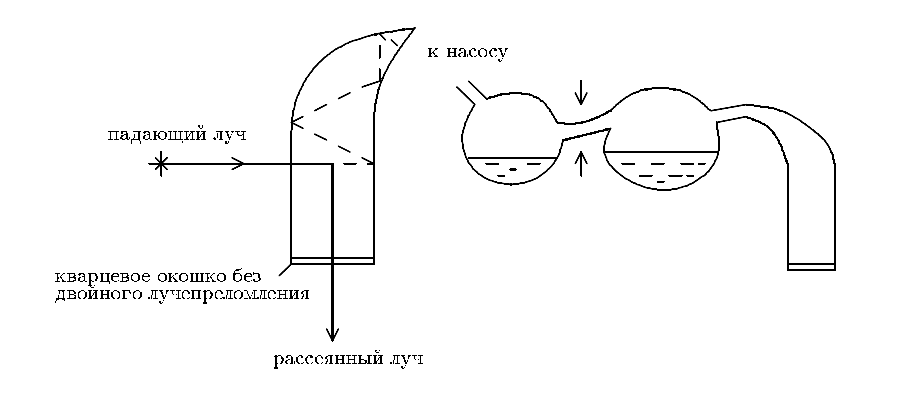
\includegraphics[scale=0.8]{Ris/ris_eps/ris4_1_11.eps}}}

\risp{1.11}{
Трубка Вуда и установка
для процедуры Мартина и Лермана}
\end{figure}

2. Соблюдать
строгую геометрию опыта, строгость в установке пентапризм,
проверке поляризаторов, а в качестве источника излучения лучше
использовать лазер.

\noindent\hangindent 1cm\hangafter 4
3. проверка входного и выходного окошка на отсутствие двойного
лучепреломления. Для изготовления окошек можно использовать
плавленый кварц, отжигая готовые изделия.
\subzag{Коэффициент рассеяния и коэффициент экстинкции}
Константа лорда Релея (коэффициент рассеяния) характеризует
абсолютную способность вещества (т. е. исключается
геометрия опыта, величина рассеивающего объема и расстояние до
точки наблюдения). С ее помощью можно сравнивать
светорассеивающую способность различных веществ.
$$R={I_{90}\cdot r^2\over I_0V}.\noq$$
Величину $R$ нередко называют абсолютной интенсивностью, а также
приведенной интенсивностью. Для коэффициента рассеяния
естественного света формулы \eqn{42} и \eqn{54} приводят к
следующим выражениям:
$$R={2\pi^2\over\lambda^4}{(n-1)^2\over N_0}\cdot
{6+6\Delta\over6-7\Delta},\noq$$
$$R={8\pi^4\over\lambda^4}N_0(\lambda^2+{13\over45}\gamma^2).\noq$$

Мы дадим три определения константы $R$, которые используются при
экспериментах: визуальном (фотографическом) и фотоэлектрическом.

1. Коэффициент рассеяния численно равен освещенности, получаемой
от 1 ${\rm см}^2$ рассеивающего объема, перпендикулярно падающему
лучу на расстоянии 1 см при 1 единице освещенности падающего
света.

2. $Ir^2$ --- сила света: световой поток, исходящий от
рассеивающего объема внутри единицы телесного угла; если его разделить
на $V$, то ${Ir^2\over V}$ --- световой поток, исходящий от
единицы рассеивающего объема в единицу телесного угла. $I_0$ ---
световой поток, падающий на единицу поверхности рассеивающего
объема. $R={I_{90}\over I_0V}$ --- доля светового потока,
падающего на единицу поверхности рассеивающего объема, которая
рассеивается единицей объема в единицу телесного угла под
$\Theta=90^{\circ}$.

3. $V=l\cdot S$; $Ir^2$ --- световой поток от площади $S$ (см.
рис. 4.1.12).
Яркость этой поверхности $b={I\cdot r^2\over S}$, тогда
$$R={b\cdot
S\over I_0Sl}={b\over I_0l}.\noq$$
Если $B$ --- яркость падающего пучка, то создаваемая им
освещенность
$$I_0=B\Omega,\noq$$
где $\Omega$ --- телесный угол, под которым падающий пучок
собирается в центре рассеивающего объема. При фотографической
регистрации освещенность фотопластинки пропорциональна яркости.
Человеческий глаз сравнивает яркости.

\begin{figure}[tbp]
\centerline{\hbox{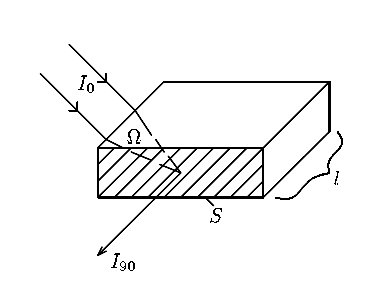
\includegraphics[scale=0.9]{Ris/ris_eps/ris4_1_12.eps}}}

\risp{1.12}{
Рассеяние света под
прямым углом от объема $V=Sl$}
\end{figure}

Подставив \eqn{59} в \eqn{58}, получаем:
$$R={b\over B\Omega l}.\noq$$
Эта формула, используется при фотографической и визуальной
регистрации.

Часто вместо $R$ пользуются другой величиной, называемой
коэффициентом экстинкции (или мутностью) $\tau$.
Если $K$ --- коэффициент поглощения:
$$I=I_0e^{-(K+\tau)l}.$$
<<Вдали>>\ от полосы
поглощения ослабление пучка света происходит только за счет
рассеяния. однако это утверждение неверно, так как даже вдали от
полосы поглощения в чистых прозрачных жидкостях, например, $\tau$
и $K$ --- величины одного порядка. Но вернемся пока к определению
$\tau$.

При прохождении света через среду
интенсивность проходящего пучка света $I_0$ постепенно
ослабляется вследствие рассеяния. 
В малых толщинах ослабление пропорционально толщине слоя
$-dI_0=\tau I_0dx$, где $\tau$ --- коэффициент экстинкции.
$$\tau=-{dI_0\over I_0dx}.\noq$$
Мы видим, что $\tau$ имеет ту же размерность, что и $R$. На
основании этой формулы можно дать следующее
определение: коэффициент экстинкции показывает,
на какую долю убывает интенсивность параллельного пучка света
при прохождении через единицу толщины рассеивающей среды.
Можно сказать иначе: $\tau$ --- это число, которое показывает,
какая часть светового потока, падающего на 1 $\rm
см^{2}$ рассеивается в слое толщиной в 1 см.
Сравнив его с аналогичным определением $R$ (пункт 2), мы можем сказать, что
если бы рассеяние было одинаковым по всем направлениям, то
$\tau$ было бы в $4\pi$ больше $R$.
Однако рассеяние света зависит от угла рассеяния по
косинусному закону. Найдем в этом случае для изотропных молекул
связь между $R$ и $\tau$.

\begin{figure}[tbp]
\centerline{\hbox{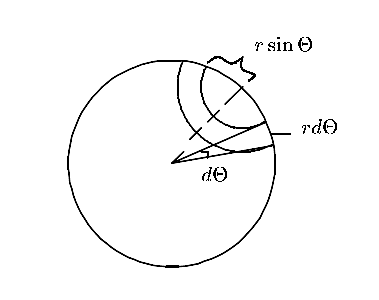
\includegraphics[scale=0.9]{Ris/ris_eps/ris4_1_13.eps}}}

\risp{1.13}{
К расчету коэффициента
экстинкции}
\end{figure}

Рассеивающий объем помещен в центр сферы радиуса $r$ (см. рис.
4.1.13). Кольцевой
элемент $dS=2\pi r\sin\Theta rd\Theta$, $\Theta$ --- угол
рассеяния. Через элемент $dS$ рассеивается световой поток
$dF$:
$$dF=I_0{8\pi^4\over\lambda^4r^2}N_0V\alpha^2(1+\cos^2\Theta)\cdot
2\pi r^2\sin\Theta d\Theta.\noq$$
Интегрируем по всем углам рассеяния от $\Theta=0$ до
$\Theta=\pi$:
$$\int\limits_{0}^{\pi}(1+\cos^2\Theta)\sin\Theta
d\Theta=\int\limits_0^{\pi}[d\cos\Theta+d{1\over3}\cos^3\Theta]=$$ $$=
\int\limits_{0}^{\pi}\cos\Theta+\int\limits_0^{\pi}{1\over3}\cos^3\Theta=
2+{2\over3}={8\over3},$$
и получаем:
$$F=I_0{128\pi^5\over3\lambda^4}N_0V\alpha^2.\noq$$
Из нашего определения $\tau$ следует, что $\tau={F\over(I_0V)}$,
отсюда:
$$\tau={128\pi^5\over3\lambda^4}N_0\alpha^2={32\pi^3\over3\lambda^4}{(n-1)^2\over
N_0}.\noq$$
Мы видели, что $R={2\pi^2\over\lambda^4}\cdot{(n-1)^2\over N_0}$,
а если $\Delta=0$, то для оптически изотропных молекул
$$\tau={16\pi\over3}R.\noq$$
Для $\Delta\not=0$ необходимо интегрировать выражение
$$I_0{8\pi^4\over\lambda^4r^2}N_0V\left\{\alpha^2(1+\cos^2\Theta)+\gamma^2
\left({13\over45}+{1\over45}\cos^2\Theta\right)\right\}.$$
Проведя необходимые вычисления, получаем:
$$R={8\pi^4\over\lambda^4}N_0(\alpha^2+{13\over45}\gamma^2),\noq$$
и, согласно \eqn{65}:
$$\tau={128\pi^5\over3\lambda^4}N_0(\alpha^2+{2\over9}\gamma^2)
={32\pi^3\over3\lambda^4}{(n-1)^2\over
N_0}\cdot{6+6\Delta\over6-7\Delta}.\noq$$
Если же  $\Delta\not=0$, то
$$\tau={16\pi\over3}R\cdot{1+0,5\Delta\over1+\Delta}.\noq$$
Соотношения \eqn{65} и \eqn{68} справедливы не только для газов,
но также для изотропных конденсированных сред --- жидкостей и
растворов. Это связано с тем, что коэффициент деполяризации чисто
анизотропного рассеяния всегда равен 6/7 для случая естественного
падающего света. Из формулы \eqn{68} следует, что отношение
$\tau/R$ имеет наибольшую величину, когда молекулы изотропны
$(\Delta=0)$.

Для нахождения ослабления пучка света в более толстых слоях уже
нельзя пользоваться дифференциальной зависимостью, а необходимо
перейти к интегральной форме
$$I_0(x)=I_0e^{-\tau x}.$$
Вблизи поверхности земли к молекулярному рассеянию света
добавляется рассеяние на мелких взвешенных частицах, которое
может оказаться в несколько раз больше молекулярного рассеяния.
\subzag{Опытное определение интенсивности рассеяния в газах}
Первые опытные исследования рассеяния света в газах в
лабораторных условиях были проведены в 1915-1920 гг. Кабанном во
Франции и Релеем в Англии 
, и затем, в некоторых
других лабораториях.

В первых опытах в качестве источника света использовалась дуговая
лампа. Рассеянный под прямым углом свет регистрировался
фотопластинкой. Ж. Кабанн и многие другие исследователи
использовали ртутную дуговую лампу. Ч. Раман и другие индусские
исследователи, а также П. Дор использовали солнце как источник
падающего света.

Сравнение относительных интенсивностей рассеяния света различных
газов показало, что при одинаковых упругостях интенсивность
рассеяния света пропорциональна квадрату рефракции $(n-1)^2$ в
соответствии с формулой Релея \eqn{56}.

Определение относительных интенсивностей рассеяния света в газах
представляет собой довольно трудную задачу. Еще более
значительные трудности возникают при определении абсолютных
интенсивностей, т. е. коэффициентов рассеяния. Здесь приходится
сравнивать два световых потока --- падающего и рассеянного
излучения, которые отличаются по яркости в миллионы или сотни
миллионов раз. Точное сравнение таких световых потоков потребовало
разработки особой методики фотометрирования. Первое определение
абсолютной интенсивности рассеяния света в газах (аргоне)
выполнил Ж. Кабанн в 1921 г. П. Дор усовершенствовал
методику измерения и в 1925 г. измерил коэффициент рассеяния
света в этилхлориде.

\begin{figure}[tbp]
\centerline{\hbox{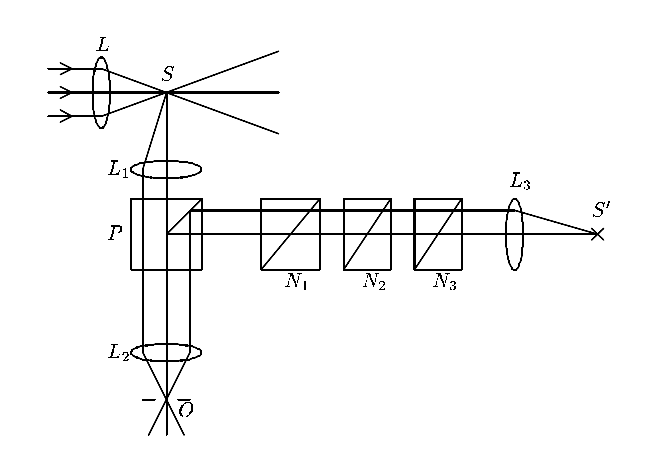
\includegraphics[scale=0.9]{Ris/ris_eps/ris4_1_14.eps}}}

\risp{1.14}{
Схема установки Дора для
измерения интенсивности рассеяния света}
\end{figure}

Этот газ рассеивает свет в 20 раз
сильнее, чем аргон. Кроме того, вместо ртутной лампы, которой
пользовался Ж. Кабанн, П. Дор использовал в качестве источника
света солнце. Все это привело к значительному повышению
интенсивности светорассеяния, так что измерения можно было
проводить не только фотографированием рассеянного излучения, но и
прямым визуальным наблюдением. На рис. 4.1.14 изображена схема
установки П. Дора. Лучи от солнца направляются с помощью
гелиостата на линзу $L$, которая собирает их внутри сосуда с
газом в точке $S$. На пути лучей от солнца стоят еще не указанные
на рисунке кювета с водой для удаления инфракрасных лучей,
могущих вызвать нагревание испытуемого газа, и другие
светофильтры для выделения из солнечного спектра узкого
спектрального участка $\lambda=520\div550$ нм. Рассеянные лучи из
точки $S$ направляются с помощью линзы $L$ параллельным пучком
через кубик Люмера $P$, а затем второй линзой $L_2$ собираются в
точке $O$, где помещается фотографическая пластинка или глаз
наблюдателя. Сбоку помещается вспомогательный источник света
$S'$, который посылает лучи через поляризационные призмы (николи)
$N_1$, $N_2$, $N_3$ на тот же кубик Люмера P, а оттуда на
выходное отверстие $O$. Призма $N_1$ поляризует лучи от
вспомогательного источника света, а другие две призмы $N_2$ и
$N_3$ позволяют ослабить эти лучи до яркости рассеянного
излучения. В принципе можно было бы обойтись одной призмой $N_2$,
но так как яркости двух сравниваемых пучков света отличаются в
очень большое число раз, то для повышения точности измерения
ставят две призмы.

Перед экспериментатором стоял прежде всего задача измерить
отношение яркости рассеянного излучения, исходящего из точки $S$,
к яркости падающего излучения. Измерение происходило в два
приема. Сначала измерялось отношение яркости рассеянного
излучения $b$ к яркости вспомогательного источника света $B'$:
$b/B'$. После этого сосуд с газом убирался и на его место
ставилась призма полного отражения, которая направляла падающий
световой поток на выходное отверстие $O$. Поворотом призм $N_2$ и
$N_3$ снова выравнивались две яркости и определялось отношение
$B'/B$, где $B$ --- яркость падающего излучения. Для получения
искомого отношения $b/B$ достаточно было умножить первое
отношение на второе.

После того, как отношение $b/B$ измерено, остается еще найти
телесный угол $\Omega$, под которым падающие лучи собираются в
точке $S$. Очевидно, $\Omega={\pi D^2\over4F^2}$, где $D$ ---
диаметр линзы, $F$ --- ее фокусное расстояние. Глубина
рассеивающего объема $l$ равна ширине изображения, создаваемого
падающим пучком света в точке $S$. Эта величина определялась
следующим образом: удалялся сосуд с газом и на его место в точку
$S$ помещалась фотографическая пластинка перпендикулярно пучку
падающего света. Измерив длину почерневшего участка, получали
$l$. Подставив все эти числа в \eqn{60}, находили $R$. Дор
получил для этилхлорида при давлении 750 мм. рт. ст. и
$19^{\circ}$ C и $\lambda_{\rm
эфф.}=530,0$ нм $R=(1,06\pm0,1)\cdot10^{-7}\ {\rm см^{-1}}$.
Измерение абсолютной интенсивности светорассеяния газа позволяет
определить число Авогадро. Дор получил
$N_A=(6,5\pm0,6)\cdot10^{23}$. В пределах точности измерения это
число находится в согласии с современным значением.

После измерения абсолютной интенсивности рассеяния света в
этилхлориде определение интенсивности светорассеяния других газов
можно свести к сравнению отношения интенсивности светорассеяния
испытуемого газа и этилхлорида. Почти одновременно с П. Дором
аналогичные исследования провел С. Ивинг с насыщенными
парами ряда соединений. Экспериментальные данные о коэффициенте
деполяризации газов и паров, а также об оптической анизотропии
молекул полно изложены в монографиях.
\vfil
\eject
\zagp{Рассеяние света в жидкостях}

\subzag{Термодинамическая теория}
Плотность жидкостей в 1000 раз больше плотности газов, однако
интенсивность рассеяния больше всего в тридцать раз, т. е.
${R_{\rm ж}\over N_1^{\rm ж}}<{R_{\rm газа}\over N_1^{\rm
газа}}$. Это результат интерференции вторичных волн, испускаемых
диполями, индуцированными световой волной в молекулах жидкости.

Применение статистической термодинамики с расчету интенсивности
света, рассеянного в конденсированных изотропных средах,
справедливо, если средняя длина пробега молекулы $\overline{l}$
много меньше длины волны света в среде $\lambda/n$. Если
выполнено условие $\overline{l}\ll\lambda/n$, то среду можно
считать непрерывной и характеризовать некоторой оптической
диэлектрической проницаемостью $\varepsilon_0$. Тепловое движение
молекул среды приводит к возникновению флуктуаций плотности и
ориентаций анизотропных молекул, которые, в свою очередь,
вызывают флуктуации оптической диэлектрической проницаемости.
Диэлектрическая проницаемость среды складывается из
$\varepsilon_0$ и малой добавки $\Delta\varepsilon$, вызванной
флуктуациями.

Если изотропная в целом среда состоит из анизотропных молекул, то
вследствие флуктуаций их взаимных ориентаций во флуктуирующем
объеме появится анизотропия, и поэтому $\Delta\varepsilon$
становится тензорной величиной
$$\varepsilon_{ik}=\varepsilon_{\sigma}\delta_{ik}+\Delta\varepsilon_{ik},\noq$$
где $\delta_{ik}$ --- единичный фактор Кронекера [см. приложение
C]. Первый член в \eqn{1} определяет значение диэлектрической
проницаемости в однородной среде, в которой рассеяние света
отсутствует, поэтому он дальше не рассматривается.

Эффект рассеяния определяется только значением
$\Delta\varepsilon_{ik}$, которое удобно представлять в виде двух
частей
$$\Delta\varepsilon_{ik}=\Delta\varepsilon\delta_{ik}+\Delta\varepsilon'_{ik},\noq$$
$$\hbox{где}\ \ \sum\limits_{i=1}^{n}\Delta\varepsilon'_{ii}=0.$$
Флуктуации $\Delta\varepsilon$ изотропны и определяются только
флуктуациями давления $\Delta p$ и энтропии $\Delta S$ или
плотности $\Delta\rho$ и температуры $\Delta T$, или любой другой
пары независимых термодинамических переменных. Флуктуации
$\Delta\varepsilon$ не нарушают изотропии среды, и поэтому свет,
рассеянный вследствие флуктуаций $\Delta\varepsilon$, должен быть
полностью поляризован. Флуктуации $\Delta\varepsilon'_{ik}$
определяют возникшую в результате теплового движения анизотропию
среды, и поэтому свет, рассеянный на $\Delta\varepsilon'_{ik}$
должен быть деполяризован. Флуктуации $\Delta\varepsilon'_{ik}$
--- флуктуации анизотропии и не могут рассматриваться в рамках
равновесной термодинамики.

Как было показано в \S 1, плодотворная идея Смолуховского (1908
г.) о флуктуациях как о причине рассеянного света легла в основу
статистической теории рассеяния света, развитой Эйнштейном.
Рассматривая $\Delta\varepsilon$ как функцию пары независимых
переменных $(\rho, T)$, т. е.
$$\Delta\varepsilon=\Delta\varepsilon(\rho,
T)=\left({\partial\varepsilon\over\partial\rho}\right)_{T}\Delta\rho+\left(
{\partial\varepsilon\over\partial T}\right)_{\rho}\Delta T.\noq$$
Эйнштейн положил $\left({\partial\varepsilon\over\partial
T}\right)_{\rho}\Delta T\simeq0$, как величину малую по
сравнению с первым членом, тогда
$$\overline{(\Delta\varepsilon)}=\left({\partial\varepsilon\over\partial\rho}\right)^2
\overline{(\Delta\rho)^2}.\noq$$
В этой же работе были вычислены средние квадратичные флуктуации
плотности и концентрации $\overline{(\Delta\rho)^2}$ и
$\overline{(\Delta C)^2}$. Впоследствии М. А. Леонтовичем было
выполнено обширное исследование флуктуаций термодинамических
величин. В приложении I приводятся необходимые формулы из
этой работы. Учитывая \eqn{4} и что
$$\overline{(\Delta\rho)^2}={1\over V}\beta_{T}kT\rho^2, \noq$$
получаем классическую формулу Эйнштейна для интенсивности
естественного света, рассеянного на расстоянии $r$ от
рассеивающего объема $V$:
$$I=I_0{\pi^2Vv^*\over2\lambda^4R^2}\left(\rho{\partial\varepsilon\over\partial
\rho}\right)^2_T\beta_T kT(1+\cos^2\theta),\noq$$
где $\theta$ --- угол рассеяния, $v^*$ --- физически малый объем.
Физическая сущность явления заключается на суммировании света,
рассеянного отдельными пространственно-независимыми флуктуациями
в физически малых объемах $v^*$. Пусть на физически малый объем
$v^*$ падает линейно поляризованный свет. Электрический вектор
падающей волны $\vec E=\vec E_0\cos(\omega t)$. Дипольный момент
единицы объема
$$\vec P={\varepsilon-1\over4\pi}\vec E.\noq$$
Очевидно, что флуктуации $\Delta\varepsilon$ вызывают
дополнительную поляризацию в единице объема
$$\Delta\vec P={\Delta\varepsilon\over4\pi}\vec E.\noq$$
Причиной рассеяния в этом случае будет флуктуация дипольного
момента в объеме флуктуации $v^*$
$$\Delta p=p-\overline{p}={\Delta\varepsilon\over4\pi}v^*E.$$
Напряженность электрического поля рассеянной волны
$$e=E{4\pi^2\over\lambda^2r}{\Delta\varepsilon\over4\pi}v^*\sin\Phi,\noq$$
где $\Phi$ --- угол между вектором $\vec E$ и радиус-вектором в
точку наблюдения $\vec r$. Интенсивность света, рассеянного
объемом $v^*$:
$$i=\overline{e^2}=I_0{\pi^2\over\lambda^4r^2}\overline{(\Delta\varepsilon)^2}v^*
\sin\Phi.\noq$$
Из статистической независимости флуктуаций плотности в двух
объемах $v^*_1$ и $v^*_2$ вытекает, что свет, рассеянный этими
объемами будет некогерентен, а следовательно можно суммировать
интенсивности света, рассеянного на отдельных объемах $v^*$
внутри рассеивающего объема $V$
$$I=I_0{\pi^2\over\lambda^4r^2}\overline{(\Delta\varepsilon)^2}Vv^*\sin^2\Phi.\noq$$
Для естественного света
$$I=I_0{\pi^2\over2\lambda^4r^2}\overline{(\Delta\varepsilon)^2}v^*V(1+\cos^2\theta),\eqno
(2.11a)$$
где $\theta$ --- угол рассеяния.

Л. И. Фабелинский показал,
что формула Эйнштейна учитывает два вида флуктуаций плотности:
адиабатические флуктуации плотности, связанные с флуктуациями
давления $\Delta p$ и изобарические флуктуации энтропии.
Рассмотрим для этого зависимость флуктуации плотности от пары
термодинамических статистически независимых переменных,
соответствующих условиям задачи: $p$ и $S$.
$$
\Delta\rho=\Delta\rho(p, S),\ \hbox{причем}\ \
\overline{(\Delta p\Delta S)}=0,\noq
$$ $$
\overline{(\Delta\rho)^2}=\left({\partial\rho\over\partial
p}\right)^2_S\overline{(\Delta p)^2}+\left({\partial\rho\over\partial
S}\right)^2_p\overline{(\Delta
S)^2}.\noq
$$
Первый член выражения \eqn{13} характеризует адиабатические
флуктуации плотности, а второй --- изобарические флуктуации
плотности. Из \eqn{11$a$}, \eqn{4} и \eqn{13} ясно, что выражение
для интенсивности рассеянного света распадается на две части
$$I=v^*G\left[\left({\partial\varepsilon\over\partial\rho}\right)^2_{T}
\left({\partial\rho\over\partial p}\right)^2_{S}\overline{(\Delta
p)^2}+\left({\partial\varepsilon\over\partial\rho}\right)^2_{T}
\left({\partial\rho\over\partial S}\right)^2_{p}\overline{(\Delta
S)^2}\right],\noq$$
$$\hbox{где}\ \
G\equiv{\pi^2V\over2\lambda^4r^2}(1+\cos^2\theta).$$
Таким образом, интенсивность света, рассеянного на адиабатических
флуктуациях плотности, равна
$$I_{ad}=v^*G\left(\rho{\partial\varepsilon\over\partial\rho}\right)^2_{T}
\left({1\over\rho}{\partial\rho\over\partial p}\right)^2_{S}\overline{(\Delta
p)^2}.\noq$$
Из статистического расчета (см. приложение I)
$$\overline{(\Delta p)^2}=-kT\left({\partial p\over\partial
V}\right)_S={kT\over\beta_Sv^*},\noq$$
и в соответствии с определением
$$\left({1\over\rho}{\partial\rho\over\partial
p}\right)_S=-{1\over V}\left({\partial V\over\partial
p}\right)_S=\beta_S.\noq$$
Тогда из \eqn{15}, \eqn{16} и \eqn{17} получаем
$$I_{ad}=G\left(\rho{\partial\varepsilon\over\partial\rho}\right)^2_T
\beta_SkT.\noq$$
Найдем интенсивность рассеянного света на изобарических
флуктуациях плотности $I_{is}$. Для $\overline{(\Delta S)^2}$
статистическая термодинамика дает (см. приложение I)
\begin{plain}
$$\eqalign{
\overline{(\Delta S)^2}=&kC_p\rho v^*,\cr
\left({1\over\rho}{\partial\rho\over\partial S}\right)_p=&
{1\over V}\left({\partial V\over\partial S}\right)_p=-{T\over
C_pv^*}\left({1\over V}{\partial V\over\partial T}\right),\cr
}\noq$$
\end{plain}
и для интенсивности света, рассеянного на изобарических
флуктуациях плотности
$$I_{is}=v^*G\left(\rho{\partial\varepsilon\over\partial\rho}\right)^2_{T}
{1\over\rho}\left({\partial\rho\over\partial
S}\right)^2\overline{(\Delta S)^2}.\eqno (2.19a)$$
учитывая \eqn{19}, получим
$$I_{is}=G\left(\rho{\partial\varepsilon\over\partial\rho}\right)_{T}^2
{kT^2\sigma^2\over C_p\rho},\noq$$
где $\sigma$ --- коэффициент объемного расширения
$\sigma=\left({1\over T}{\partial V\over\partial T}\right)_p$.
Суммируя \eqn{18} и \eqn{20} найдем
$$I=I_{ad}+I_{is}=GkT\left(\rho{\partial\varepsilon\over\partial\rho}\right)_{T}^2
\left(\beta_S+{T\sigma^2\over\rho C_p}\right).\noq$$
Так как $$\beta_T=\beta_S+{T\sigma^2\over\rho C_p},\noq$$
получим формулу Эйнштейна. Как было показано выше, формула
Эйнштейна учитывает оба вида флуктуаций плотности, но при выводе
Эйнштейн пренебрег величиной
$\left({\partial\varepsilon\over\partial T}\right)_{\rho}\Delta
T$. Проведем последовательный расчет флуктуации
$\Delta\varepsilon$ как функции энтропии и давления
$$\Delta\varepsilon(p,S)=\left({\partial\varepsilon\over\partial
p}\right)_S\Delta p+\left({\partial\varepsilon\over\partial
S}\right)_p\Delta S.$$
В силу независимости $p$ и $S$ при статистическом усреднении
получим
$$|\Delta\varepsilon(p,S)|^2=\left({\partial\varepsilon\over\partial
p}\right)^2_S\overline{\Delta p^2}+\left({\partial\varepsilon\over\partial
S}\right)^2_p\overline{\Delta S^2}.\noq$$
Мы видели, что
$$I_{ad}\sim\left({\partial\varepsilon\over\partial
p}\right)^2_{S}\overline{\Delta p^2}\ \ и
I_{is}\sim\left({\partial\varepsilon\over\partial
S}\right)^2_{p}\overline{\Delta S^2}.\noq$$
Используя соотношения, связывающие производные термодинамических
величин, получим
$$\left({\partial\varepsilon\over\partial S}\right)_p=
\left({\partial\varepsilon\over\partial T}\right)_p
\left({\partial T\over\partial S}\right)_p,\ \hbox{а}\ \ {
\partial S\over\partial T}={C_p\rho v^*\over T},\noq$$
тогда выражение \eqn{23} запишется теперь так:
$$|\Delta\overline{\varepsilon(p,S)}|^2=
\left({\partial\varepsilon\over\partial
p}\right)^2_S\overline{\Delta p^2}+
\left({\partial\varepsilon\over\partial T}\right)^2_p{T\over
C_p\rho v^*}\overline{\Delta S^2}.\noq$$
Принимая во внимание \eqn{16}, \eqn{17} и \eqn{19}, и учитывая
что
$$\left({\partial\varepsilon\over\partial p}\right)_S=
\left(\rho{\partial\varepsilon\over\partial
\rho}\right)_S\beta_S,\noq$$
получаем при статистическом усреднении
$$|\Delta\overline{\varepsilon(p,S)}|^2=
\left(\rho{\partial\varepsilon\over\partial
\rho}\right)^2_S\beta_SkT{1\over v^*}+
\left({1\over\sigma}{\partial\varepsilon\over\partial
T}\right)_p^2{\sigma^2kT^2\over
C_p\rho v^*}.\noq$$
Подставив \eqn{28} в формулу \eqn{11$a$}, получим
$$I=G\left[
\left(\rho{\partial\varepsilon\over\partial
\rho}\right)^2_S\beta_SkT+
\left({1\over\sigma}{\partial\varepsilon\over\partial
T}\right)_p^2{\sigma^2kT^2\over
\rho C_p}\right].\noq$$
В отличие от \eqn{18} и \eqn{20}, точная формула приводит к
следующим значениям $I'_{ad}$ и $I'_{is}$:
$$
I'_{ad}=G\left(\rho{\partial\varepsilon\over\partial
\rho}\right)^2_S\beta_SkT, \noq$$ $$
I'_{is}=G\left({1\over\sigma}{\partial\varepsilon\over\partial
T}\right)_p^2{\sigma^2kT^2\over
\rho C_p}. \noq
$$
Можно показать [4], что в пренебрежении величиной
$\left({\partial\varepsilon\over\partial T}\right)_{\rho}\Delta
T$, формула Эйнштейна применима, если
$\left({\partial\varepsilon\over\partial T}\right)_{\rho}{\sigma
T\over C_v\beta_T\rho}\ll\left(\rho
{\partial\varepsilon\over\partial \rho}\right)_{T}$. Правая часть
неравенства близка к 1, левая составляет приблизительно 0,02.
Более подробные оценки, основанные на экспериментальных
величинах, входящих в формулы, даны в монографии И. Л.
Фабелинского [4].


\subzagl{Приближенные формулы для расчета интегральной
интенсивности рассеянного света в жидкости}
\markright{\hfill\small 
Приближенные формулы для расчета интегральной
интенсивности 
\hfill}
Для вычисления рассеивающей способности жидкостей,
характеризуемой константой Рэлея
$$R={I_{90}\cdot r^2\over
I_0V}=kT\beta_T\left(\rho{\partial\varepsilon\over\partial\rho}\right)^2{\pi^2\over2\lambda^4},\noq$$
где $I_{90}$ --- интенсивность рассеяния под углом 90$^{\circ}$,
$V$ --- рассеивающий объ\"ем, $I_0$ интенсивность падающего
света, $\beta_T=\beta_S+{\sigma^2T\over\rho C_p}$ ---
изотермическая сжимаемость, $\beta_S={1\over\rho v^2}$ ---
адиабатическая сжимаемость, где $v$ --- скорость звука.
Необходимо рассчитать производную
$\partial\varepsilon/\partial\rho$. Считая справедливым для
жидкости уравнение Лорентц --- Лоренца, Эйнштейн
продифференцировал его и получил
$$\overline{\rho}{\partial\varepsilon\over\partial\rho}=(\varepsilon-1)^2
{\varepsilon+2\over3}\equiv(n^2-1){n^2+2\over3}.\noq$$
Однако, рассчитанная интенсивность рассеянного света для
большинства жидкостей на 40\% превышает экспериментальное
значение. И. Рокар подверг убедительной критике соотношение
\eqn{33} Эйнштейна. Уравнение Лорентц --- Лоренца связывает
показатель преломления с плотностью в состоянии равновесия, и
может и не соблюдаться при отклонениях от этого состояния.
Поэтому простое дифференцирование здесь неправомерно. Заменим в
уравнении Лорентц --- Лореца
$${\varepsilon-1\over\varepsilon+2}={4\pi\over3}N_1\alpha\noq$$
$N_1$ на ${dN\over dV}$ и перепишем его в форме
$$dV\left({\varepsilon-1\over4\pi}\right)=\alpha\left(1+{\varepsilon-1\over3}\right)dN,\noq$$
где $dN=N_1dV$ в среднем равновесном состоянии.
В левой части \eqn{35} стоит дипольный момент объ\"ема $dV$ для
напряженности поля, равной единице. $\alpha dN$ --- есть также
момент объема $dV$, но в отсутствие поляризации,
$\alpha{\varepsilon-1\over3}dN$ выражает момент, создаваемый этим
полем. При наличии отклонений от среднего соотношение перепишется
форме
$$dV\left({\bar\varepsilon-1\over4\pi}+{\partial\varepsilon\over4\pi}\right)=
\alpha\left(1+{\bar\varepsilon-1\over3}\right)(N_1dV+\Delta
dN).\noq$$
Здесь ${\bar\varepsilon-1\over3}$ в правой части уравнения
\eqn{36} не флуктуирует, так как $\bar\varepsilon$ представляет
собой среднюю диэлектрическую постоянную объема, содержащего
весьма большое число молекул.
Получаем
$$dV{\Delta\varepsilon\over4\pi}=\alpha{\bar\varepsilon+2\over3}\Delta
dN.\noq$$
Подставляя $\alpha$ из уравнения Лорентц --- Лоренца имеем
$$\Delta\varepsilon=(\varepsilon-1){\Delta dN\over\alpha
V}\cdot{1\over N_1}\ \ {\rm или}\ \
\Delta\varepsilon=(\varepsilon-1){m\over\bar\rho}{1\over
m}\Delta\rho,\noq$$
откуда
$${\partial\varepsilon\over\partial\rho}\bar\rho=\varepsilon-1\equiv
n^2-1.\noq$$
К сходным выводам приходит и Раманатан, считающий, что
следует пользоваться не уравнением Лорентц --- Лоренца, а
уравнением
$$\varepsilon-1=\hbox{const}\cdot\rho,\noq$$
так как фактор $\varepsilon+2$ возникает благодаря присутствию
окружающей молекулу среды, свойства которой не изменяются при
флуктуациях внутри данного элемента объема.

Интенсивность рассеянного света в случае подстановки выражения
\eqn{39} и \eqn{40} оказывается на 20\% меньше экспериментальных
значений. Следует отметить, что вышеуказанные приближения для
равных показателей преломления жидкостей дают различное
расхождение с опытом в зависимости от величины $n$.

Прямые измерения
$\partial\varepsilon\over\partial\rho=2n{\partial
n\over\partial\rho}$ требуют серьезных экспериментальных навыков,
поэтому чаще измеряют ${\partial n\over\partial\rho}$:
$$\left(\rho{\partial\varepsilon\over\partial\rho}\right)_T={2n\over\beta_T}
\left({\partial n\over\partial p}\right)_T.$$
Для получения требуемой точности нужен большой диапазон давлений
$p$. В качестве примера можно привести работы Гиббсона и
Кинкайзда и Дайфорса.

В работе [7] произведены измерения показателя преломления и
удельного объема бензола в широком диапазоне давлений для длин
волн $\lambda=5461\angst$ и $\lambda=4358\angst$ при температурах
25$^{\circ}$C, 35$^{\circ}$C и 45$^{\circ}$C. Авторы показали,
что удельная рефракция, вычисленная по формуле Эйкмана 
$$r={n^2-1\over n+0,4}\cdot{1\over\rho}\noq$$
остается постоянной при всех давлениях и температурах. Величина
производной
$\left(\rho{\partial\varepsilon\over\partial\rho}\right)_T$ может
быть вычислена из этих экспериментальных данных. Дифференцируя
\eqn{41}, находим
$$\left(\rho{\partial\varepsilon\over\partial\rho}\right)_{T}=
{n^2-1\over1-{n^2-1\over2n(n+0,4)}}.\noq$$
Использование формулы \eqn{42} при расчете константы рассеяния
бензола приводит к хорошему согласию с экспериментальными
данными. Подобные расчеты были произведены для сероуглерода в
работе [8], где была получена зависимость $\varepsilon=f(\rho)$
при изменении давления от 1 до 1000 атмосфер при температуре
350$^{\circ}$C и $450^{\circ}$C.

Сложность экспериментов в работах [7], [8] привела исследователей
к поиску хорошо обоснованной теоретически формулы для вычисления
$\left(\rho{\partial\varepsilon\over\partial\rho}\right)_T$.
Такое исследование было проведено Ивоном в его статистической
теории рассеяния света. Расчет $R$ по формуле Ивона для
всех жидкостей независимо от величины показателя преломления дает
согласие с экспериментом не хуже 1\%.
\subzag{Тонкая структура линии рассеяния}
Выше рассматривалось рассеяние света, вызванное неоднородностями
показателя преломления, возникающими в свою очередь вследствие
различных тепловых флуктуаций. При выводе формул в каждом случае
отыскивались величины соответствующих флуктуаций, но не
рассматривались их изменения во времени. Такой подход вполне
обоснован, если искать суммарную интенсивность рассеяния, не
затрагивая вопроса о спектральном составе рассеянного света.

Действительно, предполагалось, что в некотором объеме находится
определенное при данной температуре количество локальных
оптических неоднородностей (флуктуаций показателя преломления),
не зависящие от времени, а сами они считаются <<застывшими>>.
В этом случае была найдена зависимость суммарной интенсивности
рассеянного света от измеряемых на опыте параметров среды и длины
волны падающего света.

Рассеянный свет имеет при этом ту же длину волны, что и
возбуждающий, если возбуждающий свет монохроматичен. Если же
возбуждение рассеяния осуществляется участком непрерывного
спектра, то распределение интенсивности в рассеянном свете буде
изменено в соответствии с законом $I\sim{1\over\lambda^4}$. В
действительности статистические флуктуации не остаются <<
застывшими>>, а непрерывно меняются во времени. Флуктуации
характеризуют отклонение от равновесного состояния, и поэтому они
неустойчивы.

Различные флуктуации по-разному меняются во времени и поэтому
различным образом модулируют рассеянный свет. То обстоятельство,
что каждый вид флуктуаций налагает свой характерный <<
отпечаток>> на спектр рассеянного света, позволяет использовать
спектры рассеянного света для изучения кинетики флуктуаций. Выше
исследовалась интенсивность света, рассеянного на флуктуациях
плотности.

Ниже будут кратко рассмотрены те изменения, которые вносятся в
спектр рассеянного света временными изменениями флуктуаций
плотности и концентрации. Как уже было указано выше, флуктуации
плотности складываются из адиабатических флуктуаций (флуктуации
давления) и изобарических флуктуаций (флуктуации энтропии).
Флуктуации давления представляют собой случайные локальные сжатия
или разрежения, которые вследствие упругих свойств среды не
остаются на месте, но <<бегут>>\ по объему вещества.
Многочисленные случайные сжатия и разрежения, возникающие
вследствие тепловых флуктуаций давления, можно рассматривать как
упругие волны различных частот, распространяющиеся по
всевозможным направлениям внутри изучаемого объема.

Напомним, что при расчете суммарной интенсивности рассеянного
света Эйнштейн разлагал флуктуацию плотности в пространственный
ряд Фурье и по статическим амплитудам разложения отыскивал
интенсивность рассеянного света.

Изучая вопросы теплоемкости твердого тела Дебай в своей работе
пришел к плодотворной идее о том, что энергию, приходящуюся
на все $3N$ степеней свободы связанных атомных осцилляторов
твердого тела, можно рассматривать как энергию $3N$ нормальных
упругих волн. Таким образом, Дебай рассматривает энергию
теплового движения твердого тела как энергию упругих волн. С этой
точки зрения флуктуации есть результат интерференции дебаевских
волн.

Мы дадим краткие сведения о теории теплоемкости кристаллического
твердого тела. Классическая теория теплоемкости твердого
тела приводит к закону Дюлонга и Пти
$$C_v=3R\simeq6\ \hbox{кал/моль}.\noq$$
Этот закон выводится, как известно, следующим образом.
Предполагается равномерное распределение энергии по степеням
свободы. Каждая частица в кристалле обладает тремя степенями
свободы, на каждую из них приходится средняя кинетическая
энергия, равная ${kT\over2}$, всего ${3\over2}kT$. Однако,
частица в кристалле обладает не только кинетической, но и
потенциальной энергией, зависящей от смещения частицы из ее
положения равновесия
$$U=U(r-r_0).$$
Разлагая это выражение в ряд по малым смещениям около положения
равновесия, имеем
\begin{plain}
$$\eqalign{
U=&U_0+\left({\partial U\over\partial
r}\right)_{r=r_0}(r-r_0)+\cr
+&{1\over2}\left({\partial^2 U\over\partial
r^2}\right)_{r=r_0}(r-r_0)+\ldots,\cr
}\noq$$
\end{plain}
причем, так как в положении равновесия потенциальная энергия
имеет минимум, линейный член в \eqn{33} равен нулю. Ограничиваясь
малыми смещениями, мы можем считать $U$ квадратичной функцией
смещений и, следовательно, силу, действующую на частицу, линейной
функцией смещения
$$f=-{\partial U\over\partial r}=-\left({\partial^2
U\over\partial r^2}\right)_{r=r_0}(r-r_0).\noq$$
Именно это предположение лежит в основе теории упругости.
Находясь под действием упругой возвращающей силы, каждая частица
в кристалле выполняет гармоническое колебание --- является
гармоническим осциллятором. Как известно, средняя потенциальная
энергия гармонического осциллятора равна его средней кинетической
энергии. Всего, следовательно, на каждую частицу приходится
энергия, равная
$$\overline{E}={3\over2}kT+{3\over2}kT=3kT$$
и на $N_A$ частиц (один моль) $3RT$. Следовательно, теплоемкость
$$C_v={\partial\overline{E}\over T}=3R,\noq$$
т. е. закон Дюлонга и Пти. Однако этот закон соблюдается при
комнатной температуре далеко не для всех кристаллов, а при низкой
температуре не соблюдается вовсе. Согласно \eqn{34} $C_v$ не
зависит от температуры. В действительности, при низких
температурах $C_v$ резко понижается, стремясь к значению $C_v=0$
при $T\rightarrow0^{\circ}$ K (третье начало термодинамики). Для
объяснения зависимости теплоемкости твердого тела от температуры,
Эйнштейн воспользовался идеей Планка, согласно
которой излучение твердого тела квантовано. Эйнштейн предположил,
что твердое тело представляет собой, в соответствии с изложенным,
систему осцилляторов, но каждый осциллятор имеет квантованную
энергию, может приобретать тепловую энергию отдельными квантами,
равными $\hbar\omega$. Как мы знаем сейчас, энергия осциллятора
$${\cal E}_n=\left(n+{1\over2}\right)\hbar\omega,\noq$$
где $n=0,\ 1,\ 2,\ 3\ \ldots$

Согласно основным положениям статистической физики, вероятность
состояния осциллятора с энергией ${\cal E}_n$ равна
$$\overline{{\cal E}}={\sum\limits_{n=0}^{\infty}{\cal
E}_ne^{-{{\cal E}_n\over kT}}\over
\sum\limits_{n=0}^{\infty}e^{-{{\cal E}_n\over kT}}}={\cal E}_0+
{\sum\limits_{n=0}^{\infty}n\hbar\omega e^{-{n\hbar\omega\over kT}}\over
\sum\limits_{n=0}^{\infty}e^{-{n\hbar\omega\over kT}}},\noq$$
где ${\cal E}_0$ --- нулевая энергия, равная
${\hbar\omega\over2}$. Произведя суммирование, находим
$$\overline{{\cal E}}={\hbar\omega\over2}+{\hbar\omega\over
e^{{\hbar\omega\over kT}}-1}.\noq$$
Тело, состоящее из $N$ частиц, имеет $3N$ степеней свободы и
энергию, равную
$$\overline{{\cal E}}=3N{\hbar\omega\over2}+{3N\hbar\omega\over
e^{{\hbar\omega\over kT}}-1}.\noq$$

\begin{figure}[tbp]
\centerline{\hbox{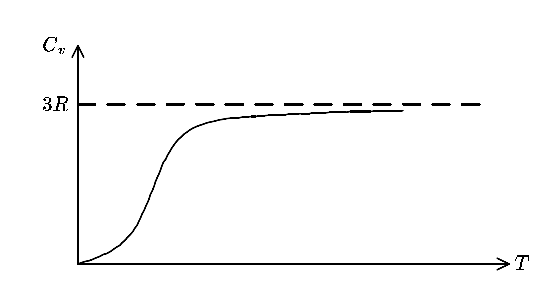
\includegraphics[scale=0.9]{Ris/ris_eps/ris4_2_01.eps}}}

\risp{2.1}{
Кривая теплоемкости
твердого тела}
\end{figure}

Теплоемкость $C_v$ равна
$$C_v={\partial\overline{{\cal E}}\over\partial
T}={3N(\hbar\omega)^2e^{{\hbar\omega\over kT}}\over k^2
T(e^{{\hbar\omega\over kT}}-1)^2}.\noq$$
При высоких температурах, удовлетворяющих условию
$kT\gg\hbar\omega$, получаем по-прежнему $C_v=3Nk$.

Температурный ход $C_v$ \eqn{39} показан на рис. 4.2.1. В
действительности, как показывает опыт, кривая $C_v(T)$ медленнее
приближается к нулевому значению вблизи абсолютного нуля
температуры и, что самое существенное, твердое тело нельзя
охарактеризовать какой-то одной единственной частотой упругих
колебаний $\omega$. Мы видели, что упругие свойства твердого тела
достаточно сложны и существенно зависят от его симметрии. Мы
должны рассматривать колебания всех частиц твердого тела, как
связанные. Потенциальная энергия всей совокупности частиц
кристалла должна зависеть не только от квадратов смещений
отдельных частиц из положений равновесия, но и от произведений
смещений различных частиц, так как силы, действующие на данную
частицу, зависят от смещений соседних частиц.

Мы можем, однако, по-прежнему представить энергию системы как
сумму энергий гармонических осцилляторов, соответствующих
отдельным нормальным колебаниям системы, общее число которых
равно числу степеней свободы системы, т. е. $3N$. В каждом
нормальном колебании принимают участие все частицы системы.

Мы имеем право пользоваться для отдельного нормального колебания
прежним выражением \eqn{37}
$${\cal E}_k={\hbar\omega_k\over2}+{\hbar\omega_k\over
e^{{\hbar\omega_k\over kT}}-1}\noq$$
и находим, что средняя энергия кристалла равна
$$\overline{{\cal E}}=\sum\limits_{k=1}^{3N}\overline{{\cal
E}}_k={\cal E}_0+\sum\limits_{k=1}^{3N}{\hbar\omega_k\over
e^{{\hbar\omega_k\over kT}}-1},\noq$$
где
$${\cal E}_0={\hbar\over2}\sum\limits_{k=1}^{3N}\omega_k.\noq$$
Задача, таким образом, сводится к вычислению частот всех
нормальных колебаний системы. Это --- очень трудная задача. Дебай
нашел ее решение для непрерывного изотропного тела,
характеризуемого двумя упругими постоянными для поперечного и
продольного сжатия.

Рассмотрим специфические особенности рассеяния света на
флюктуациях плотности в сплошной (кристаллической или аморфной)
среде. Теория соответствующих явлений была разработана Л. И.
Мандельштамом.

Рассмотрим, следуя за Л. И. Мандельштамом, какова будет
дифракционная картина, полученная при прохождении плоской
световой волны через слегка оптически неоднородную среду. Эти
неоднородности будем считать вызванными распространяющимися в
среде упругими возмущениями. Как мы видели, упругие возмущения в
кристалле могут быть представлены звуковыми волнами, образующими
дебаевские ветви в спектре кристаллической решетки. Л. И.
Мандельштам вводит два предположения:

1) что изменение показателя преломления среды $\delta n$
обусловливается только изменением плотности среды $\delta \rho$ и
пропорционально $\delta \rho$. При этом $\delta n$ --- малая
величина и мы имеем право пренебречь ее квадратом и высшими
степенями;

2) что за время наблюдения вс\"е возмущение заключено в
ограниченной замкнутой области, целиком находящейся в поле
зрения.

Оба эти предположения соответствуют реальным свойствам среды.
Второе предположение исходит из факта относительной медленности
распространения звуковых волн
$${\partial (\delta\rho)\over\rho\partial t}\ll{c\over l}\ \
\hbox{или}\ \ v\ll c$$
($c$ --- скорость света, $v$ --- скорость звука, $l$ --- линейные
размеры области возмущения в направлении $x$ распространения
волны). Отсюда следует, что интерференционную картину можно
рассчитывать, как статистическую, т. е. не учитывая изменений
$\delta \rho$, происходящих за время прохождения световой волны
через область возмущения.

Вычислим амплитуду (комплексную) результирующего электрического
вектора рассеянного света в точке, отстоящей на расстоянии $R$ от
области возмущения.
$$\widetilde{E}_0=A\int\delta n\cdot e^{ik(R-x)}d\tau.\noq$$
Интегрирование распространяется на область, целиком включающую
область возмущения, $k={2\pi\over\lambda}$, $A$ --- константа.
Нас интересует зависимость $\widetilde{E}_0$ от времени. Так как
$\delta\rho$ подчиняется волновому уравнению (звуковая волна)
$${\partial^2\delta\rho\over\partial
t^2}=v^2\nabla^2\delta\rho\noq$$
и, согласно предположению 1), $\delta n\sim \delta \rho$, имеем
$${\partial^2\delta n\over \partial t^2}=v^2\nabla^2\delta n.\noq$$
Дважды дифференцируя \eqn{44} по $t$ и подставляя \eqn{46},
находим
$${\partial\widetilde{E}_0\over\partial
t^2}=Av^2\int\nabla^2\delta n\cdot e^{ik(R-x)}d\tau.\noq$$
Преобразуем интеграл \eqn{47} на основании теоремы Грина. Для
любых двух функций $\varphi$ и $\psi$
$$\int(\nabla^2\varphi\cdot\psi-\nabla^2\psi\cdot\varphi)d\tau=\int\left(
\varphi{\partial\psi\over\partial
N}-\psi{\partial\varphi\over\partial N}\right)dS.$$
Интеграл в правой части берется по поверхности, охватывающей
область интегрирования, в подынтегральном выражении фигурируют
производные по нормали к поверхности. Принимая $\varphi=\delta n$
и $\psi=e^{ik(R-x)}$, получаем
$$\int(\nabla^2\delta n\cdot e^{ik(R-x)}-\nabla^2
e^{ik(R-x)}\cdot \delta n)d\tau=\int\left(\delta n{\delta
e^{ik(R-x)}\over\partial N}-e^{ik(R-x)}{\partial\delta
n\over\partial N}\right)dS$$
и, так как согласно предположению 2), на границе области
возмущения
$$\delta n={\partial\delta n\over\partial N}=0,$$
преобразуем \eqn{37} к виду
$${\partial^2\widetilde{E}_0\over\partial t^2}=Av^2\int\nabla^2
e^{ik(R-x)}\cdot\delta n\cdot d\tau.$$
Имеем
$$\nabla^2
e^{ik(R-x)}=-4k^2\sin^2{\theta\over2}e^{ik(R-x)}+2{ik\over
R}e^{ik(R-x)},$$
где $\theta$ --- угол между направлениями $R$ и $x$. На
раcстояниях $R\gg\lambda$ второй член много меньше первого и им
можно пренебречь. Следовательно,
$${\partial^2\widetilde{E}_0\over\partial
t^2}=-4k^2v^2A\sin^2{\theta\over2}\int\delta n\cdot
e^{ik(R-x)}d\tau\noq$$
или, согласно \eqn{34}
$${\partial^2\widetilde{E}_0\over\partial
t^2}=-4k^2v^2\sin^2{\theta\over2}\widetilde{E}_0,\noq$$
откуда
$$\widetilde{E}_0=B_1e^{i\Omega t}+B_2e^{-i\Omega t},\noq$$
где
$$\Omega=2vk\sin{\theta\over2}=2\omega{v\over
c}\sin{\theta\over2}.$$
Полное выражение для волны
$$E=\widetilde{E}_0 e^{i\omega t}=B_1 e^{i(\omega+\Omega)t}+B_2
e^{i(\omega-\Omega)t}.$$
Таким образом, в спектре рассеянного света присутствуют частоты,
отличные от частоты падающего света.

При монохроматическом падающем свете, свет рассеянный содержит
дублет с частотами
$$\omega'=\omega\left(1\pm2{v\over c}\sin{\theta\over2}\right).\noq$$
Расщепление
$${\delta\omega\over \omega}={\delta\nu\over\nu}=\pm2{v\over
c}\sin{\theta\over2} \noq$$
тем больше, чем больше отличается направление рассеяния от
направления падающей волны. При $\theta=0$, $\delta\omega=0$.

Полученный результат \eqn{51} может быть выведен и истолкован при
помощи следующих простых рассуждений.

Как уже сказано, тепловое движение в твердых телах, в результате
которого возникают флюктуации плотности $\delta\rho$, сводится к
наложению дебаевских гиперзвуковых волн с частотами порядка
$10^{12} \hbox{ --- } 10^{18}$ герц. Мы можем рассматривать эти волны, как
стоячие или как бегущие. В первом случае задача исследования
свойств света, рассеянного средой, сводится к изучению рассеяния
на системе стоячих волн, сгущений и разрежений, образующих
пространственную дифракционную решетку. Очевидно, что такая
задача вполне аналогична задаче о дифракции рентгеновских или
электронных волн кристаллической решеткой. Различие состоит в
том, что в последнем случае рентгеновы лучи рассеиваются
неподвижной дискретной системой натуральных точек --- атомов или
ионов, а в нашей задаче решетка синусоидальная и колеблется со
со звуковой частотой.

В общих случаях отражение --- рассеяние света должно происходить
только в определенных направлениях, удовлетворяющих условию
Брэгга-Вульфа:
$$2d\sin{\theta\over2}=m\lambda.\noq$$

\begin{figure}[tbp]
\centerline{\hbox{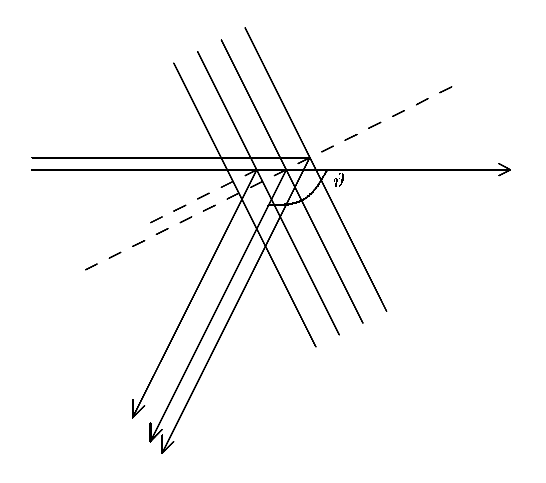
\includegraphics[scale=0.9]{Ris/ris_eps/ris4_2_02.eps}}}

\risp{2.2}{
Дифракция на стоячих
волнах}
\end{figure}

Здесь $d$ --- постоянная решетки, $\theta$ --- угол между
направлением падающего и рассеянного света, $\lambda$ --- длина
волны света, $m=1,\ 2,\ 3,\ \ldots$ --- дает нам порядок
дифракционного спектра. Соотношение \eqn{53} легко вывести с
помощью рис. 4.2.2. Однако, как это было показано Рэлеем, для
синусоидальной решетки возможен только спектр первого порядка, т.
е. $m=1$. Следовательно, должно соблюдаться условие
$$2d\sin{\theta\over2}=\lambda.$$
Роль постоянной решетки играет длин звуковой волны $\Lambda$.
Имеем
$$2\Lambda\sin{\theta\over2}=\lambda,\noq$$
откуда соответствующая рассеянию света частота звуковой волны
равна
$$\Omega={2\pi v\over\Lambda}={4\pi
v\over\lambda}\sin{\theta\over2}=2\omega{v\over
c}\sin{\theta\over2}.\noq$$
Вследствие периодического изменения флюктуации плотности
$\delta\rho$ во времени, получаем для напряженности
электрического поля рассеянной световой волны
\begin{plain}$$\eqalign{
E^S\sim
E^0\delta\varepsilon=&E^0{\partial\varepsilon\over\partial\rho}\delta\rho=
E^0_0\cos\omega
t{\partial\varepsilon\over\partial\rho}\delta\rho=\cr
=&{\partial\varepsilon\over\partial\rho} E_0^0\cos\omega t\cdot
(\delta\rho)_0\cos\Omega
t=\cr
=&{1\over2}{\partial\varepsilon\over\partial\rho}(\delta\rho)_0E_0^0\{\cos(\omega+\Omega)t+
\cos(\omega-\Omega)t\},\cr
}\noq$$
\end{plain}
причем частота $\Omega$ удовлетворяет условию \eqn{55}. Мы
получили дублет с частотами $\omega\pm\Omega$. Очевидно, что
физическая причина расщепления при рассмотрении явления на
стоячих волнах сводится к модуляции световой волны по амплитуде
звуковыми колебаниями.

\begin{figure}[tbp]
\centerline{\hbox{\includegraphics[scale=0.9]{Ris/ris_eps/ris4_2_03.eps}}}

\risp{2.3}{
Отражение от
движущегося зеркала}
\end{figure}


К тому же результату мы придем, рассматривая рассеяние света как
отражение от бегущих звуковых волн. В этом случае физической
причиной расщепления является эффект Доплера. В самом деле,
бегущая световая волна --- фронт сгущений плотности --- может
рассматриваться как движущееся
зеркало (рис. 4.2.3). Мы всегда
имеем две одинаковых волны --- бегущую вправо и влево. При
отражении света от движущегося зеркала происходит изменение
частоты колебаний. Имеем
$${\delta\omega\over\omega}=2{v\over c}\cos\alpha,$$
где $\alpha$ --- угол, образуемый отраженным лучом с нормалью к
зеркалу, лежащей в плоскости падения, вдоль которой направлена
скорость. Согласно рис. 4.2.3, получаем
$${\delta\omega\over\omega}=2{v\over c}\sin{\theta\over2}$$
и, так как наряду со звуковой волной, движущейся со скоростью
$+\vec v$, имеется волна, движущаяся со скоростью $-\vec v$,
имеем
$${\delta\omega\over\omega}=\pm2{v\over c}\sin{\theta\over2}.$$
Мы вновь получили прежний результат. Отсутствие расщепления в
направлении падающей волны $\theta=0$ становится совершенно
ясным в этой интерпретации: рассеяние по первоначальному
направлению происходит на упругих волнах, движущихся
перпендикулярно к направлению распространения. При этом обычный
эффект, дающий расщепление очень малой и практически не
наблюдаемой величины порядка ${v^2\over c^2}$.

Рассмотрение явления, как модуляции световых волн звуковыми
колебаниями, принадлежит Л. И. Мандельштаму. Рассмотрение на
основе эффекта Доплера было предложено Бриллюэном. Основная
формула
$$\omega'=\omega\left(1\pm2{v\over
c}\sin{\theta\over2}\right)\noq$$
носит название формулы Мандельштама --- Бриллюэна. Вследствие
того, что гиперзвуковые волны распространяются в кристалле по
любым направлениям, всегда имеется волна, удовлетворяющая условию
\eqn{55}, и свет рассеивается под любыми углами.

Экспериментальное подтверждение изложенных теоретических
соображений представляет исключительный интерес. В теории Л. И.
Мандельштама объединена теория рассеяния света жидкостями
Эйнштейна с теорией теплоемкости кристаллов Дебая. Мы уже
говорили, что Эйнштейн в своей основной работе проводил расчеты.
разлагая флюктуации плотности в ряд Фурье --- представляя их
наложением неких периодических движений, которые Эйнштейн вводил
чисто формальным образом. С другой стороны, Дебай построил теорию
теплоемкости кристалла, рассматривая тепловое движение в нем, как
гиперзвуковые волны. Л. И. Мандельштам в изложенной теории,
применимой не только к кристаллу, но и к жидкости, исходил из
того, что эйнштейновские компоненты ряда Фурье, на которых
происходит рассеяние, являются реальными дебаевскими упругими
волнами. В

\begin{figure}[tbp]
\centerline{\hbox{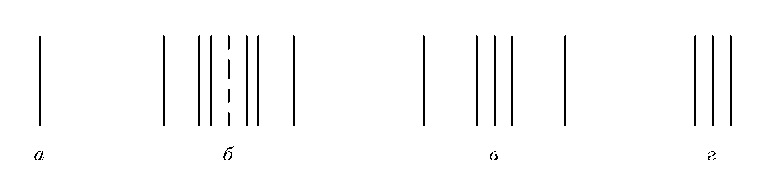
\includegraphics[scale=0.9]{Ris/ris_eps/ris4_2_04.eps}}}

\risp{2.4}{
Схема тонкой структуры
рэлеевской линии:}\vskip 1mm\centerline{\ris {\small\it а} ---
падающий свет, {\small\it б} --- кристалл, {\small\it в} --- аморфное
твердое тело, {\small\it г} --- жидкость}
\end{figure}

этом случае расщепление спектральной линии в
рассеянном свете должно наблюдаться и в кристаллах, и в
жидкостях. Как мы увидим ниже, это замечательное предсказание Л.
И. Мандельштама было подтверждено прямыми опытами.

Рассмотрим теперь, что дает экспериментальное исследование тонкой
структуры рэлеевской линии. Мы видели, что, согласно теории Л. И.
Мандельштама, рэлеевская линия в спектре рассеяния кристалла
должна представлять собой дублет. Оценим порядок величины
ожидаемого дублетного расщепления. Допустим, что кристалл кварца
освещается светом ртутной дуги с $\lambda=4358 \angst$
($\nu=7\cdot10^{14}\ {\rm сек^{-1}}$). Угол рассеяния
$\theta=90^{\circ}$. Скорость звука в кварце $\sim\ 6000$
м/сек $=6\cdot10^5$ см/сек. Имеем
$$2\Delta\nu=4\nu{v\over
c}\sin{\theta\over2}=4,7\cdot10^{14}{6\cdot10^5\over3\cdot10^{10}}{\sqrt{2}\over2}=
4\cdot10^{10}\ {\rm сек^{-1}}$$
и
$$2\Delta\lambda=2\Delta\left({c\over\nu}\right)=-2c{\Delta\nu\over\nu^2}=-
3\cdot10^{10}{4\cdot10^{10}\over49\cdot10^{28}}=0,25\angst.$$
Таким образом, ожидаемое расщепление весьма мал\'о и может быть
экспериментально обнаружено только средствами интерференционной
спектроскопии. Соответствующие опыты были, по предложению Л. И.
Мандельштама, осуществлены Е. Ф. Гроссом и подтвердили
теоретические ожидания. Преодолев трудности, связанные с
необходимостью работать с очень чистым образцом кристалла и с
поддержанием постоянной температуры всей спектрографической
установки с точностью до тысячных долей градуса, Е. Ф. Гросс смог
наблюдать предсказанное Л. И. Мандельштамом расщепление
рэлеевской линии.

При дальнейшем, более детальном исследовании, Е. Ф. Гросс
обнаружил, что в действительности рэлеевская линия расщеплена не
на две, а на шесть компонент. Эти результаты объясняются
тем, что наряду с продольной, в кристалле распространяются две
поперечные звуковые волны. Известно, что для кварца их предельные
скорости равны: для продольной 6400 м/сек, для поперечных ---
3500 и 2400 м/сек. Это объяснение может быть проверено
непосредственно. Согласно формуле \eqn{55}, скорость звуковой
волны определяется из величины расщепления следующим образом:
$$v={\Delta\cdot\lambda\over2\sin{\theta\over2}}.\noq$$
Вычисленные из секстетного расщепления значения звуковых
скоростей в кварце оказались равны, соответственно, 6800, 3800 и
3300 м/сек. Совпадение следует считать очень хорошим. Мы видим,
что изучение оптического явления --- тонкой структуры рэлеевской
линии --- позволяет исследовать акустические свойства кристалла.

В аморфном твердом теле скорости двух поперечных волн должны
совпадать и вместо секстетного должно наблюдаться квартетное
расщепление и наряду со смещенными компонентами в этом случае
должна наблюдаться и несмещенная. Наконец, в жидкостях Гросс
установил дублетное расщепление и также несмещенную
компоненту с интенсивностью того же порядка, что и компоненты
расщепления. Схематически получаемые во всех перечисленных
случаях картины могут быть представлены следующим образом (рис.
4.2.4).

Очевидно, что существование несмещенной компоненты в случаях
аморфных тел и жидкостей требует специального объяснения.
Естественно предположить, что за эту компоненту ответственны
медленно рассасывающиеся флюктуации ориентации -- анизотропии, в
кристалле невозможные. Однако, как мы увидим ниже, действительное
объяснение --- иное. Оно было дано Ландау и Плачеком,  
опубликовавшими без вывода следующую формулу, определяющую
отношение интенсивностей несмещенной компоненты и компонент
дублета:
$${I_{\omega}\over
I_{\omega+\Delta\omega}+I_{\omega-\Delta\omega}}={C_p-C_v\over
C_v},\noq$$
где $C_p$ и $C_v$ --- теплоемкости при постоянном давлении и
объеме соответственно. И за компоненту с частотой $\omega$ и за
компоненты с частотами $\omega\pm\Delta\omega$ ответственны
флюктуации плотности.

Однако распространение упругих звуковых волн есть не единственный
процесс возникновения $\Delta\rho$. В 1945 году Е. Ф. Гросс
опубликовал обоснование  формулы Ландау и Плачека.
Флуктуации плотности, или, что в сущности то же самое,
флуктуации удельного объема
$$\Delta v=\Delta{1\over\rho}=-{1\over\rho^2}\Delta\rho$$
могут быть представлены
$$\Delta v=\left({\partial v\over \partial p}\right)_S\Delta
p+\left({\partial v\over \partial S}\right)_p\Delta S.\noq$$
Первый член правой части характеризует адиабатический процесс
флуктуации давления. Эти флуктуации распространяются со скоростью
звука и именно с ними мы имеем дело в предшествующем изложении.
Напротив, второй член описывает изобарические флуктуации
энтропии. Эти флуктуации рассасываются со скоростью, определяемой
теплопроводностью вещества. Эта скорость значительно меньше
звуковой. Поэтому, в то время как флуктуации энтропии приводят
к появлению дублета (секстета), флуктуации энтропии определяют
существование несмещенной линии.

Интенсивность рассеянного света пропорциональна $\overline{\Delta
v^2}$. Так как $\overline{\Delta p\cdot\Delta S}=0$, имеем
$$\overline{\Delta v^2}=\left({\partial v\over\partial
p}\right)^2_S\overline{(\Delta p)^2}+\left({\partial v\over
\partial S}\right)^2\overline{(\Delta S)^2},\noq$$
$${I_{\rm несмещ.}\over I_{\rm дублет}}={\left({\partial v\over
\partial S}\right)^2\overline{(\Delta S)^2}\over\left({\partial
v\over \partial p}\right)^2\overline{(\Delta p)^2}}.\noq$$

Задача сводится к нахождению средних квадратичных флуктуаций
энтропии и давления. Они легко находятся методами статистической
физики. Имеем
$$\overline{(\Delta S)^2}=kC_p,\hskip 4mm\overline{(\Delta
p)^2}=-{kT\over\left({\partial v\over\partial p}\right)_S}.$$
С другой стороны, термодинамика дает
$$\left({\partial v\over\partial S}\right)_p=\left({\partial
T\over\partial p}\right)_S={T\over C_p}\left({\partial
v\over\partial T}\right)_p;\hskip 4mm \left({\partial
v\over\partial p}\right)_S={C_v\over C_p}\left({\partial
v\over\partial p}\right)_T.$$
И, наконец
$$C_p-C_v=-{T\left({\partial v\over\partial T}\right)^2_P\over
\left({\partial v\over\partial p}\right)_T},$$
откуда
$${I_{\rm несмещ.}\over I_{\rm дублет}}={C_p-C_v\over C_v}.$$
Легко понять, почему центральная компонента наблюдается в
жидкостях, но не в кристаллах. Для последних разность $C_p-C_v$
очень мала, а для жидкостей она достигает величины, соизмеримой с
$C_v$.
\def\eqnpl#1{(I.#1)}
\def\noqpl{\global\advance\numq by 1\eqno(I.\the\numq)}
\vfil
\eject
\zagp{Приложение I}
\subzag{ Нахождение флуктуаций некоторых термодинамических величин}

Пусть физическая величина $x$ может отклоняться от своего
среднего значения $\overline{x}$ на величину
$x-\overline{x}=\Delta x$, где $\Delta x$ есть флуктуация $x$.
Пусть вероятность найти значение $\Delta x$, заключенное в
интервале $d(\Delta x)$, задается распределением Гаусса:
$$W(\Delta x)d(\Delta x)=\hbox{const}\cdot\exp\left\{-{(\Delta
x)^2\over2\overline{|\Delta x|^2}}\right\}d(\Delta x),\noqpl$$
где $\overline{|x|^2}$ --- средний квадрат флуктуации физической
величины. С другой стороны, вероятность отклонения
термодинамической величины $x$ от ее равновесного значения $x_0$,
определяется принципом Больцмана:
$$W(\Delta x)d(\Delta x)=\hbox{const}\cdot\exp\left\{-{\Delta\Psi
\over kT}\right\}d(\Delta x),\noqpl$$
где $\Delta\Psi$ может быть в
разных случаях изменением свободной энергии, энтальпии,
термодинамического или химического потенциалов.

Минимальная работа $A_{\rm min}$, необходимая, чтобы обратным
образом осуществить отклонение термодинамической величины от ее
начального значения $A_{\rm min}\equiv\Delta\Psi=\Delta E-T\Delta
S+p\Delta V$.

Если рассматривать небольшие изменения $\Delta\Psi$, которые как
раз и описывают флуктуации, то обычно $\Delta\Psi$ можно
разложить в ряд Тейлора по любым двум термодинамическим
переменным и ограничиться квадратичными членами ряда.

Пусть $\Delta\Psi$ есть функция двух независимых переменных,
например энтропии $S$ и давления $p$, тогда
$$
\Delta\Psi(S,p)=\left({\partial E\over\partial
S}\right)_p\Delta S+\left({\partial E\over\partial
p}\right)_S\Delta p+{1\over2}\left\{\left({\partial^2 E\over\partial
S^2}\right)_p(\Delta S)^2+\right.$$ $$
\left.+\left({\partial^2 E\over\partial
p^2}\right)_S(\Delta p)^2+2{\partial^2E\over\partial S\partial
p}(\Delta p\Delta S)\right\}-$$ $$-T\Delta S+p\left({\partial V\over\partial
p}\right)_S\Delta p+p\left({\partial V\over\partial
S}\right)_p\Delta S,
\noq$$
где призводные взяты при равновесных значениях величин $p$ и $S$.
Сумма коэффициентов при $\Delta S$, а также сумма коэффициентов
при $\Delta p$ равны нулю. Поэтому
\begin{plain}
$$\eqalign{
\Delta\Psi(\S,p)={1\over2}\left\{\left({\partial^2 E\over\partial
S^2}\right)_p(\Delta S)^2+\right.&\left.\left({\partial^2 E\over\partial
p^2}\right)_S(\Delta p)^2+2{\partial^2 E\over\partial S\partial
p}\Delta S\Delta p\right\}=\cr
&={1\over2}\left[\Delta p\Delta\left({\partial E\over\partial
p}\right)_S+\Delta S\Delta\left({\partial E\over\partial
S}\right)_p\right].\cr
}\noq$$
\end{plain}
Учитывая, что
$$\left.\matrix{\left({\partial E\over\partial
p}\right)_S=-p\left({\partial V\over\partial
p}\right)_S,\ \left({\partial E\over\partial
S}\right)_p=T-p\left({\partial V\over\partial S}\right)_p,\cr
\left({\partial V\over\partial
S}\right)_p=\left({\partial T\over\partial
p}\right)_S,\ \Delta T=\cr
}\right\}$$
\vfil
\eject
\zagp{Рассеяние света в растворах}

\subzag{Термодинамическая теория}
У растворов появляется новый вид флуктуаций --- флуктуации
концентрации, которые дают дополнительный вклад в рассеяние
света. Флуктуации концентрации происходят независимо от
флуктуаций плотности и ориентации, поэтому полную интенсивность
рассеяния света можно представить в виде суммы трех слагаемых
$$I=I_{\rm пл}+I_{\rm к}+I_{\rm ан},$$
где $I_{\rm пл}$, $I_{\rm к}$, $I_{\rm ан}$ --- интенсивности
рассеяния света на флуктуация плотности, концентрации и
анизотропии соответственно. Так как рассеяние света на
флуктуациях анизотропии в общем случае трудно рассчитать, то мы
его будем учитывать через коэффициент деполяризации. Для угла
рассеяния $\theta=90^{\circ}$, как мы знаем из предыдущего,
оно учитывается с помощью множителя Кабанна
$$I=(I_{\rm пл}+I_{\rm к}){6+6\Delta\over6-7\Delta}.\noq$$

Перейдем к расчету интенсивности концентрационного рассеяния
. Ограничимся двухкомпонентными растворами. Рассеяние
света в растворах, как и в чистых жидкостях, обязано флуктуациям
диэлектрической проницаемости. Формулу [2.11] можно перенести
без изменения и на растворы
$$I=I_0{\pi^2\over\lambda^4r^2}\overline{(\Delta\varepsilon)^2}Vv^*\sin^2\Phi.\noq$$
где $\Phi$ --- угол между направлением электрического вектора
падающей волны и радиус-вектором в направлении распространения
рассеянной волны, $V$ --- объем, $v^*$ --- элемент объема.

Если считать молекулы изотропными, то для двухкомпонентного
раствора можно написать
$$\Delta\varepsilon={\partial\varepsilon\over\partial\rho}\Delta\rho+
{\partial\varepsilon\over\partial x}\Delta x$$
или, ввиду независимости флуктуаций концентрации и плотности,
$$\overline{\Delta\varepsilon^2}=\left({\partial\varepsilon\over\partial\rho}\right)^2
\overline{\Delta\rho^2}+\left({\partial\varepsilon\over\partial
x}\right)^2\overline{\Delta x^2},$$
где $x$ --- молярная концентрация (молярная доля) одного из
компонентов, $x_1$ --- концентрация первого компонента, $x_2$ ---
концентрация второго компонента, $x_1+x_2=1$. Если мы подставим
это в \eqn{2}, то получим интенсивность рассеяния света в виде
суммы двух слагаемых --- рассеяния на флуктуациях плотности и
рассеяния на флуктуациях концентрации. После перехода от
интенсивности к коэффициенту рассеяния будем иметь для второго
слагаемого
$$R_{\rm
к}={Ir^2\over I_0V}={\pi^2\over\lambda^4}\left({\partial\varepsilon\over\partial
x}\right)^2\overline{\Delta x^2}v^*\sin^2\Phi.$$
Последнее выражение относится к случаю поляризованного падающего
света. Чтобы перейти к естественному падающему свету, достаточно
заменить $\sin\Phi$ на $(1+\cos^2\theta)/2$, где $\theta$
--- угол рассеяния. Для рассеяния под углом
$\theta=90^{\circ}$ получаем
$$R_{\rm
к}={\pi^2\over2\lambda^4}\left({\partial\varepsilon\over\partial
x}\right)^2\overline{\Delta x^2}v^*.\noq$$

Остается рассчитать $\overline{\Delta x^2}v^*$. Обозначим через
$\Delta A$ минимальную работу, необходимую для изменения
концентрации в элементе объема $v^*$ от равновесной величины на
$\Delta x$. Тогда вероятность того, что в данном элементе объема
$v^*$, являющегося частью замкнутой системы, концентрация
изменяется на $\Delta x$, равна
$$W=W_0\exp\left(-{\Delta A\over kT}\right).\noq$$
Мы рассматриваем флуктуации концентрации при неизменной
температуре и давлении. Известно, что при подобных условиях мерой
работы является термодинамический потенциал Гиббса $G$. Работа
изменения концентрации в элементе объема равна $\Delta A=\Delta
G_{v^*}$, где $\Delta G_{v^*}$ --- термодинамический потенциал
элемента объема.

Если мы обозначим через $G_0$ и $G$ соответственно молярный
термодинамический потенциал Гиббса при равновесной концентрации
$x$ и при $x+\Delta x$, то для изменения термодинамического
потенциала Гиббса в элементе объема $v^*$ при изменении
концентрации на $\Delta x$ будем иметь
$$\Delta G_{v^*}={G-G_0\over V_{12}}v^*,\noq$$
где $V_{12}$ --- молярный объем раствора. Прежде чем подставить
выражение \eqn{5} в \eqn{4}, разложим его в ряд по степеням
$\Delta x$ около равновесного значения термодинамического
потенциала $G_0$. В равновесном состоянии он имеет минимум,
поэтому $\left({\partial G\over\partial x}\right)_{G=G_0}=0$.
Следовательно, $G-G_0={1\over2}\left({\partial^2 G\over\partial
x^2}\right)\Delta x^2+\ldots$. Пренебрегая членами более высокого
порядка, получаем
$$\Delta G_{v^*}=\Delta A={1\over2}\left({\partial^2
G\over\partial x^2}\right){v^*\over V_{12}}\Delta x^2.$$
Подставляя в \eqn{4}, получаем
$$W=W_0\exp\left(-{\Lambda\over2}\Delta x^2\right),\noq$$
где для сокращения введено обозначение $\Lambda=\left({\partial^2
G\over\partial x^2}\right){v^*\over V_{12}kT}$. Теперь можно
перейти к расчету $\overline{\Delta x^2}$. По аналогии с
предыдущими вычислениями в 2.1 можем написать
$$\overline{\Delta
x^2}={\int\limits_{0}^{\infty}\exp\left(-{\Lambda\over2}\Delta
x^2\right)\Delta
x^2dx\over\int\limits_{0}^{\infty}\exp\left(-{\Lambda\over2}\Delta
x^2\right)dx}.$$
Интегрирование дает
$$\overline{\Delta x^2}={1\over\Lambda}=RT\left(N_A{\partial^2
G\over\partial x^2}\right)^{-1}{V_{12}\over v^*},\noq$$
где $R$ --- газовая постоянная, $N_A$ --- число Авогадро.

Подставляя \eqn{5} в \eqn{3}, находим для интенсивности
концентрационного рассеяния
$$R_{\rm
к}={\pi^2\over2\lambda^4N_A}\left({\partial\varepsilon\over\partial
x}\right)^2RT\left({\partial^2 G\over\partial
x^2}\right)^{-1}_{p, T}V_{12}.\noq$$
Значки $p,T$ означают, что производная берется при постоянной
температуре и постоянном давлении (для простоты мы будем часто их
опускать). В термодинамике растворов величина $\left({\partial^2
G\over\partial x^2}\right)_{p,T}$ служит мерой стабильности
раствора против расслоения на две фазы смежного состава. В
критической точке расслоения она обращается в нуль. Очевидно, чем
меньше эта величина, тем больше флуктуации концентрации. Нам
представляется целесообразным характеризовать уровень флуктуаций
концентрации безразмерной величиной $f$ следующим образом:
$$f={x_1x_2\over RT}\left({\partial^2 G\over\partial
x^2}\right)_{p,T}.\noq$$
Как мы увидим ниже, для идеального раствора $f=1$, для растворов
с положительным отклонением от идеальности $f$ больше единицы, а
для растворов с отрицательным отклонением --- меньше единицы.

Будем называть $f$ функцией флуктуаций концентрации. Подставим
функцию $f$ в формулу \eqn{8}, тогда будем иметь
$$R_{\rm
к}={\pi^2\over2\lambda^4N_A}\left({\partial\varepsilon\over\partial
x}\right)^2x_1x_2V_{12}f.\noq$$
Нашу новую величину можно также выразить через другие
термодинамические величины: например,  через избыточный
термодинамический потенциал Гиббса $G^{E}$, или химический
потенциал $\mu$, или, наконец, через активность $a$
$$G=G_{\rm ид}+G^E.$$
Из термодинамики известно, что для идеального раствора
$${\partial^2 G_{\rm ид}\over\partial x^2}={RT\over x_1x_2},$$
поэтому вместо \eqn{9} можно написать
$${1\over f}=1+{x_1x_2\over RT}{\partial^2 G^E\over\partial
x^2}.\noq$$
Отсюда видно, что для идеального раствора $f=1$. Воспользовавшись
термодинамическим соотношением,
$$G=x_1\mu_1+x_2\mu_2$$
и известным уравнением Гиббса --- Дюгема
$$x_1\left({\partial \mu_1\over\partial
x_1}\right)_{p,T}+x_2\left({\partial\mu_2\over\partial
x_1}\right)_{p,T}=0,$$
где $\mu_1$ и $\mu_2$  --- молярные химические потенциалы
компонентов раствора, нетрудно доказать, что
$${\partial^2 G\over\partial x_1^2}={1\over x_2}{\partial
\mu_1\over\partial x_1}.$$
Подставляя в \eqn{9}, получаем третье выражение для $f$
$${1\over f}={x_1\over RT}{\partial \mu_1\over\partial
x_1}={x_1\over RT}{\partial \mu_2\over\partial x_2}.\noq$$
Для того, чтобы выразить функцию флуктуаций концентрации через
активность, воспользуемся термодинамическим соотношением
$$\mu_1=\mu_0+RT\ln a_1,$$
где $a_1$ --- активность первого компонента, $\mu_0$ ---
постоянная, равная химическому потенциалу при $a_1=1$, отсюда
получаем
$${\partial\mu_1\over\partial x_1}=RT{\partial \ln
a_1\over\partial x_1}.$$
Подставляя в \eqn{12}, получаем выражение для $f$ через
активность
$${1\over f}={\partial\ln a_1\over\partial \ln x_1}={\partial\ln
a_2\over\partial \ln x_2}.\noq$$

Формула \eqn{10} показывает, что для вычисления интенсивности
концентрационного рассеяния света в растворе необходимо знать
следующие величины: ${\partial\varepsilon\over\partial
x}=2n{\partial n\over\partial x}$, $V_{12}$ и $f$. Величина
${\partial n\over\partial x}$ определяется из наклона касательной
к выбранной точке кривой зависимости показателя преломления от
молярной доли одного из компонентов. Обычно подобная кривая
сильно отличается от прямой линии, что приводит к значительной
погрешности в определении величины ${\partial n\over \partial
x}$. Для повышения точности определения этой величины лучше всего
построить кривую зависимости показателя преломления от весовой
доли $c_1$ или $c_2$, откуда можно определить $\partial
n\over\partial c$, а затем с помощью пересчетной формулы найти
${\partial n\over\partial x}$
$${\partial n\over\partial x_1}={\partial n\over\partial
c_1}\left({c_1\over x_1}\right)^2{M_2\over M_1},\noq$$
где $M_1,\ M_2$ --- молекулярные веса компонентов смеси.
Необходимо, однако, отметить, что полученное подобным образом
макроскопическое значение ${\partial n\over\partial x}$
отличается от флуктуационного значения, входящего в формулу
\eqn{10}. Связь между этими двумя значениями будет
рассматриваться ниже.

Вторая величина --- молярный объем раствора $V_{12}$ находится по
формуле
$$V_{12}={M_{12}\over\rho}={x_1M_1+x_2M_2\over\rho},$$
где $M_{12}$, $\rho$ --- молекулярный вес и плотность раствора
соответственно. В тех случаях, когда при смешивании двух
жидкостей не происходит заметного отклонения объема раствора от
суммы объемов, $V_{12}$ можно определить по аддитивной схеме
$V_{12}=x_1V_1+x_2V_2$, где $V_1$, $V_2$ --- молярные объемы
компонентов.

Наибольшую трудность представляет определение термодинамической
величины $f$. Согласно формуле \eqn{9} определение этой величины
сводится к изучению термодинамических свойств раствора в
зависимости от концентрации. Но ее можно определить и
непосредственно из концентрационной зависимости упругости пара.
Так как химический потенциал молекул в жидкой фазе такой же, как
и в паре, то, приняв пар за идеальный газ, можно написать
$\mu_1=\mu_{10}+RT\ln p_1$, где $\mu_1$ --- химический потенциал
первого компонента в паре над раствором; $\mu_{10}$ ---
постоянная. Аналогичным образом можно написать для второго
компонента $\mu_2=\mu_{20}+RT\ln p_2$. Возьмем производные по
концентрации ${\partial \mu_2\over\partial x_1}=RT{\partial
p_1\over p_1\partial x_1}$, ${\partial\mu_2\over\partial
x_2}=RT{\partial p_2\over p_2\partial x_2}$ и подставим в
\eqn{12}, тогда получаем новое выражение для функции $f$
$${1\over f}={x_1\over p_1}{\partial p_1\over\partial
x_1}={x_2\over p_2}{\partial p_2\over\partial x_2}.\noq$$
Мы видим, что эту величину можно определить непосредственно из
кривой концентрационной зависимости парциального давления. Для
идеального раствора справедлив закон Рауля
$$p_1=p_{10}x_1,\hskip 4mm p_2=p_{20}x_2,$$
где $p_{10}$, $p_{20}$ --- упругости пара над чистыми
компонентами. Возьмем производные ${\partial p_2\over\partial
x_1}={p_1\over x_1}$, ${\partial p_2\over\partial x_2}={p_2\over
x_2}$ и подставим в \eqn{15}, тогда получаем $f=1$. Таким
образом, для идеального раствора при всех концентрациях $f$ равна
единице. При очень малых концентрациях все растворы близки к
идеальным растворам, так как парциальное давление растворенного
вещества растет пропорционально концентрации $x_2$, а
парциальное давление растворителя понижается пропорционально
уменьшению концентрации $x_1$, точно так же, как в идеальном
растворе. Поэтому при очень слабых концентрациях как первого, так
и второго компонента $f=1$. Отсюда следует, что функция $f$
всегда начинается со значения $f=1$ при $x_2=0$ и кончается
значением $f=1$ при $x_2=1$.

Функцию $f$ можно связать с осмотической сжимаемостью
$$\beta_{\rm осм}=\left({\partial x_2\over x_2\partial
\Pi}\right),$$
где $\Pi$ --- осмотическое давление. Осмотическая сжимаемость
является аналогом обычной изотермической сжимаемости $\beta_T$.
Можно показать, что 
$$\beta_{\rm осм}=f{x_1\over x_2}{V_1\over RT}.$$
Если мы заменим в формуле \eqn{10} $f$ на $\beta_{\rm осм}$, то
для интенсивности концентрационного рассеяния получаем новое
выражение
$$R_{\rm к}={\pi^2\over2\lambda^4}kT\beta_{\rm
осм}\left(x_2{\partial \varepsilon\over\partial
x_2}\right)^2{V_{12}\over V_1},\noq$$
которое по форме очень похоже на выражение для интенсивности
рассеяния света на флуктуациях плотности.

В предыдущем параграфе было обращено внимание на то, что значение
величины $\partial\varepsilon/\partial\rho$ зависит от того,
происходит ли изменение диэлектрической проницаемости во всем
объеме жидкости или внутри малого элемента объема. В данном
параграфе приводится аналогичное рассмотрение для
$\partial\varepsilon/\partial x$.

{\it Оптическая поляризация раствора.}\hskip 4mm Обозначим через
$\alpha_1$ и $\alpha_2$ поляризуемости молекул компонентов смеси,
а через $N_1$ и $N_2$ --- их число в 1 $\rm см^{3}$ раствора
. Тогда для вектора поляризации можно будет написать два
выражения --- одно через макроскопическую величину $\varepsilon$,
другое --- через молекулярные $\alpha_1$, $\alpha_2$
$$P={\varepsilon-1\over4\pi}E,\hskip 4mm
P=(\alpha_1N_1+\alpha_2N_2)F,\noq$$
где $\varepsilon=n^2$ --- оптическая диэлектрическая
проницаемость смеси, $F$ --- напряженность действующего поля:
$$F={\varepsilon+2\over3}E.\noq$$

Сделаем два предположения: 1) допустим, что молярные объемы двух
компонентов смеси $V_1$ и $V_2$ одинаковы (это означает, что
$N_A/V_1=N_A/V_2=N_0$); 2) пусть при образовании смеси не
происходит изменения объема --- объем смеси в точности равен
сумме объемов компонентов. Первое предположение не имеет
принципиального значения. От него мы потом легко освободимся.
Второе предположение является существенным во всем ходе наших
рассуждений.

Из наших предположений следует, что при всех изменениях
концентрации число молекул в единице объема не меняется
$$N_1+N_2=N_0={\rm const},\hskip 4mm \Delta N_1+\Delta N_2=0.\noq$$
При небольших изменениях концентрации из формул \eqn{17} получаем
два выражения для вариации поляризации
$$\Delta
P={\Delta\varepsilon\over4\pi}E+{\varepsilon-1\over4\pi}\Delta E,$$
$$\Delta P=(\alpha_1-\alpha_2)\Delta
N_1F+(\alpha_1N_1+\alpha_2N_2)\Delta F.\noq$$
Применим эти формулы к двум частным случаям: концентрация
изменяется во всем макроскопическом объеме раствора; концентрация
меняется только в малом сферическом элементе объема,
находящегося внутри большого объема раствора.

{\it Макроскопическое изменение концентрации.}\hskip 4mm Мы
исходим из условия, что внешнее поле $E$ в объеме диэлектрика
задается, поэтому ни о какой зависимости этого поля от
$\varepsilon$ говорить не приходится. Но действующее поле $F$
меняется в соответствии с изменением $\varepsilon$ по формуле
\eqn{18}, поэтому в данном случае, когда изменяется
диэлектрическая проницаемость всего раствора, имеем
$$\Delta E=0,\hskip 4mm \Delta F={\Delta\varepsilon\over3}E.$$
Вместо \eqn{20} можем написать
$$\Delta P={\Delta\varepsilon\over4\pi}E,\hskip 4mm \Delta
P=(\alpha_1-\alpha_2)\Delta
N_1{\varepsilon+2\over3}E+(\alpha_1N_1+
\alpha_2N_2){\Delta\varepsilon\over3}E.$$
Сравнивая эти два выражения получаем
$${\partial\varepsilon\over\partial
N}=(\varepsilon+2){{4\over3}\pi(\alpha_1-\alpha_2)\over1-{4\over3}\pi(\alpha_1N_1+
\alpha_2N_2)}.\noq$$
С помощью формулы Лорентц -- Лоренца для чистых компонентов
преобразуем числитель формулы \eqn{21}
$${4\over3}\pi(\alpha_1-\alpha_2)={1\over
N_0}\left({\varepsilon_1-1\over\varepsilon_1+2}-{\varepsilon_2-1\over
\varepsilon_2+2}\right).\noq$$
Для преобразования знаменателя воспользуемся формулой Лорентц ---
Лоренца для раствора
${\varepsilon-1\over\varepsilon+2}={4\over3}\pi\alpha_1N_1+{4\over3}\pi\alpha_2N_2$
или
$$1-{4\over3}\pi(\alpha_1N_1+\alpha_2N_2)=1-{\varepsilon-1\over\varepsilon+2}=
{3\over\varepsilon+2}.\noq$$
Подставляя \eqn{22} и \eqn{23} в \eqn{21}, получаем
$${\partial\varepsilon\over\partial N_1}={\varepsilon+2\over
N_0}\left({\varepsilon_1-1\over\varepsilon_1+2}-{\varepsilon_2-1\over\varepsilon_2+2}\right)
{\varepsilon+2\over3}.\noq$$

Остается еще перейти от числа молекул в единице объема $N_1$ и
$N_2$ к объемным концентрациям $\varphi_1$ и $\varphi_2$. Если мы
примем во внимание наши два условия, то можем написать
$$N_1=N_0\varphi_1,\ \ N_2=N_0\varphi_2,\ \ \Delta
N_1=N_0\Delta\varphi_1.$$
Заменим в формуле \eqn{24} $\Delta N_1$ на $N_0\Delta\varphi_1$,
тогда получаем окончательно
$$\left({\partial\varepsilon\over\partial\varphi_1}\right)=(\varepsilon
+2)\left({\varepsilon_1-1\over\varepsilon_1+2}-{\varepsilon_2-1\over\varepsilon_2
+2}\right){\varepsilon+2\over3}.\noq$$

Полученную формулу легко обобщить на случай, когда молярные
объемы компонентов неодинаковы. Пусть молярный объем второго
компонента в $m$ раз меньше, чем первого $V_1=mV_2$. Обозначим
через $\alpha_2$ поляризуемость небольшого коллектива из $m$
молекул второго компонента, а через $N'_2$ --- их число в 1 $\rm
см^3$ раствора $\alpha'_2=m\alpha_2$, $N'_2=N_2/m$. Тогда
по-прежнему можем написать
$$N_1+N'_2=N_0=\hbox{const},\ \ \Delta N_1+\Delta N'_2=0$$
и весь предыдущий вывод остается неизменным, если мы везде
заменим $\alpha_2$ на $\alpha'_2$ и $N_2$ на $N'_2$. Но если мы
также учтем, что
$$\alpha'_2N'_2=\alpha_2N_2,\ \ {4\over3}\pi(\alpha_1-\alpha'_2)=
{1\over
N_0}\left({\varepsilon_1-1\over\varepsilon_1+2}-{\varepsilon_2-1\over
\varepsilon_2+2}\right),$$
то снова приходим к формуле \eqn{25}. Таким образом, формула
\eqn{25} остается справедливой во всех случаях, независимо от
молярных объемов компонентов смеси. Необходимым условием
справедливости этой формулы является сохранение объема при
смешении.

{\it Изменение концентрации внутри малой сферы.}\hskip 4mm Здесь
мы рассматриваем флуктуационное изменение диэлектрической
проницаемости в малом сферическом элементе объема, лежащего
внутри большой массы раствора. Эти флуктуации вызывают отклонение
поля $E$ от его среднего значения. Изменение $\varepsilon$ на
$\Delta\varepsilon$ сопровождается отклонением поля от его
среднего значения на величину $\Delta
E=-{\Delta\varepsilon\over3\varepsilon}E$. Иначе обстоит дело с
действующим полем $F$. Предположим здесь так же, как и в
параграфе 2, что действующее поле не испытывает флуктуации, тогда
при флуктуационных изменениях концентрации будем иметь:
$$\Delta E=-{\Delta\varepsilon\over3\varepsilon}E,\ \ \Delta F=0$$
и вместо \eqn{20} получаем
$$\Delta
P={\Delta\varepsilon\over4\pi}E-{\varepsilon-1\over4\pi}{\Delta\varepsilon\over
3\varepsilon}E,\ \ \Delta P=(\alpha_1-\alpha_2)\Delta
N_1{\varepsilon+2\over3}E.$$
Сравнивая последние два выражения, находим
$${\partial\varepsilon\over\partial N_1}=(\varepsilon+2){4\over
3}\pi(\alpha_1-\alpha_2){3\varepsilon\over2\varepsilon+1}$$
или, заменив ${4\over3}\pi(\alpha_1-\alpha_2)$ по формуле
\eqn{22} и $\partial N_1$ на $N_0\partial\varphi_1$, получаем
$$\left({\partial\varepsilon\over\partial\varphi_1}\right)_{\rm
фл}=(\varepsilon+2)\left({\varepsilon_1-1\over\varepsilon_1+2}-{\varepsilon_2
-1\over\varepsilon_2+2}\right){3\varepsilon\over2\varepsilon+1}.\noq$$
Нет надобности доказывать, что эта формула также справедлива при
любых соотношениях молярных объемов компонентов. Единственным
условием является аддитивность объема при смешении.

Таким образом, мы нашли, что две величины
$\partial\varepsilon/\partial\varphi$ и
$(\partial\varepsilon/\partial\varphi)_{\rm фл}$ не совпадают
друг с другом. Сравнение приводит к следующему соотношению:
$$\left({\partial\varepsilon\over\partial\varphi}\right)_{\rm фл}=
\left({\partial\varepsilon\over\partial\varphi}\right){3\varepsilon\over2
\varepsilon+1}{3\over\varepsilon+2},$$
которое показывает, что первая величина меньше второй. Последнее
соотношение остается в силе при замене объемной концентрации
$\varphi$ на молярную $x$. Если заменить одновременно
$\varepsilon$ на $n^2$, то будем иметь окончательно
$$\left({\partial n^2\over\partial x}\right)_{\rm фл}=
\left({\partial n^2\over\partial
x}\right){3n^2\over2n^2+1}{3\over n^2+2}.\noq$$
Формулу \eqn{27} нельзя считать строго доказанной, так как она
выведена в предположении, что $\Delta F=0$. Поэтому в дальнейшем
значительное внимание будет уделено экспериментальной проверке
этой формулы.

Мысль о том, что флуктуационная величина производной не совпадает
с ее макроскопическим значением, не является новой. Этой идеей мы
обязаны И. Рокару. С. Багавантам предложил
соотношение
$$\left({\partial n^2\over\partial x}\right)_{\rm фл}=
\left({\partial n^2\over\partial x}\right){3\over n^2+2},$$
которое отличается от нашего отсутствием множителя
$${3n^2\over2n^2+1}$$. При выводе последней формулы не была
учтена флуктуация поля $E$.

Формула Багавантама не дает удовлетворительного согласия с
опытом. В литературе отмечалось, что если для вычисления
интенсивности светорассеяния растворов пользоваться его формулой,
то получаются заниженные значения интенсивности. С другой
стороны, было отмечено, что если вообще не делать никакого
различия между флуктуационным и макроскопическим значениями
производно2 $\partial\varepsilon/\partial x$, то, напротив,
получаются завышенные интенсивности светорассеяния растворов. М.
Дестрио, Р. Лоше и А. Руссе предложили свою формулу для
нахождения флуктуационного значения $\partial\varepsilon/\partial
x$.

Если мы подставим формулу \eqn{27} в \eqn{10}, и заменим
$\partial\varepsilon/\partial x$ на $2n\partial n/\partial x$, то
для интенсивности концентрационного рассеяния света получаем
окончательное выражение
$$R_{\rm к}={\pi^2\over2\lambda^4N_A}\left(2n{\partial
n\over\partial
x}\right)^2\left({9n^2\over(2n^2+1)(n^2+2)}\right)^2x_1x_2V_{12}f.\noq$$
\subzag{Определение функции флуктуаций концентрации из упругости
пара}
Выше мы говорили, что термодинамическую величину $f$, отражающую
уровень флуктуаций концентрации, лучше всего определять из
парциальных давлений пара. Последние обычно находят из
анализа состава пара по плотности или показателю преломления
после его конденсации. При подобного рода измерениях трудно
избежать значительных погрешностей, которые добавляются к
погрешности определения упругости пара. В дальнейшем это
обнаруживается по разбросу экспериментальных точек вокруг кривых
зависимости парциальных давлений от концентрации. В таких случаях
трудно рассчитывать на то, что значения функции $f$ будут найдены
с достаточно хорошей точностью, так как последние определяются
прежде всего наклоном касательной к соответствующей точке кривой
зависимости парциального давления от концентрации. При таком
определении $f$ два значения $f$ и $f'$, полученные из двух
кривых парциальных давлений, оказываются различными. Для того,
чтобы избежать подобной неопределенности, мы сочли более
целесообразным находить как парциальные давления $p_1$ и $p_2$,
так и функцию $f$ с помощью расчета по экспериментальной кривой
зависимости упругости пара от концентрации, без использования
каких-либо дополнительных опытных данных. Такой прием нахождения
$p_1$ и $p_2$ был предложен уже давно.

Прежде чем перейти к изложению методики расчета, введем для
удобства новые обозначения. Обозначим концентрацию первого
компонента (растворителя) через $x$ вместо $x_1$, а концентрацию
второго через $y$ вместо $x_2$. Для парциальных давлений введем
соответственно обозначения $q$ и $r$ вместо $p_1$ и $p_2$. Полное
давление пара будем обозначать через $p$. Рассматриваемый метод
заключается в том, что для нахождения двух величин $q$ и $r$ мы
используем два уравнения. Первое уравнение $q+r=p$ или $\Delta
q+\Delta r=\Delta p$. Но так как $\Delta q$ отрицательна, то
заменив ее абсолютной величиной, мы можем переписать последнее
равенство иначе
$$\Delta r=\Delta q+\Delta p.\noq$$
Второе уравнение мы получаем из формулы \eqn{15}, которую
перепишем здесь в следующем виде:
$${1\over f}={\Delta q\over\Delta x}{x\over q}={\Delta
r\over\Delta r}{y\over r}.\noq$$

Конкретно мы предлагаем следующую схему расчета. Разбиваем всю
область концентрации от 0 до 1 на большое число одинаковых
интервалов $\Delta x$. Достаточно разбить на 100 или даже 50
частей. Мы разбиваем на 50 частей. Тогда ширина элементарного
интервала концентрации будет $\Delta x=1/50$. Так как для
предельно малой концентрации, как было отмечено выше, $f=1$, то
для первого интервала концентрации, когда $x$ близка к единице, а
$y$ к нулю, мы вправе написать
$${\Delta q\over\Delta x}{x\over q}={\Delta q_1\over \Delta
x}{1\over q_0}=1$$
или взяв $\Delta x=0,02$, получаем $\Delta q_1=q_0\Delta
x=0,02q_0$, где $q_0$ --- упругость пара первого компонента.
После этого находим все числа для границы первого интервала
$$q_1=q_0-\Delta q_1=0,98q_0,\ \ \Delta r_1=\Delta q_1+\Delta
p_1,\ \ r_1=\Delta r_1,$$
$$x_1=0,98, y_1=0,02.$$
Отсюда нетрудно найти два значения $f$ для первого интервала
$$f_1={\Delta x\over\Delta q_1}{q_1\over
x_1}={0,02\over0,02q_0}\cdot{0,98q_0\over0,98}=1,$$
$$f'_1={\Delta y\over\Delta r_1}{r_1\over y_1}={0,02\over\Delta
r_1}\cdot{\Delta r_1\over0,02}=1.$$

Прежде чем перейти ко второму интервалу, найдем выражение для
$\Delta q$. Для этой цели воспользуемся уравнениями \eqn{29} и
\eqn{30}, откуда после исключения $\Delta r$ получаем
$$\Delta q={\Delta p\over{x\over q}{r\over y}-1}.\noq$$

\begin{figure}[tbp]
\centerline{\hbox{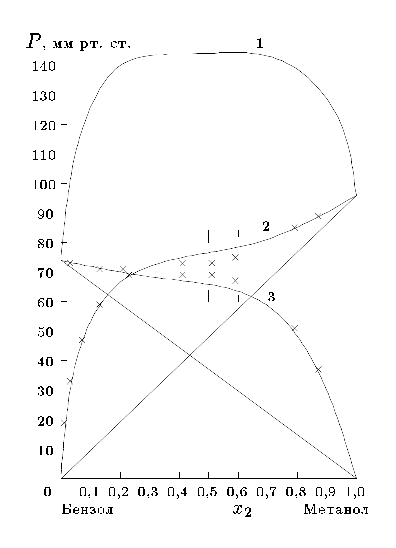
\includegraphics[scale=0.9]{Ris/ris_eps/ris4_3_01.eps}}}

\risp{3.1}{
Упругость пара (1) и парциальные
давления бен-}
\centerline{\ris \ \ \ зола (3) и метанола (2) в системе бензол---метанол при
20$^{\circ}$ C}
\vskip-5mm
\end{figure}

После этого можем написать
$$\Delta q_2={\Delta p_2\over{x_1\over q_1}{r_1\over y_1}-1},$$
$$q_2=q_1-\Delta q_2,\ \ \Delta r_2=\Delta q_2+\Delta p_2,\ \
r_2=r_1+\Delta r_2,$$
$$x_2=0,96,\ \ y_2=0,04.$$
Мы получили все числа для второго интервала. Осталось вычислить
$f_2$
$$f_2={0,02\over \Delta q_2}{q_2\over0,96},\ \
f'_2={0,02\over\Delta r_2}{r_2\over 0,04}.$$
Переходим к третьему интервалу, затем к четвертому и т. д.
Для $i+1$-го интервала получаем
$$\Delta q_{i+1}={\Delta p_{i+1}\over{x_i\over q_i}{r_i\over
y_i}-1}.\noq$$
Получаемые таким способом два значения $f$ немного отличаются
между собой. Чтобы уменьшить расхождение, можно взять более узкие
интервалы. Но в этом нет особой надобности, так как усреднение
двух чисел дает достаточно хорошее приближение к истинному
значению. Более точный, но зато более трудоемкий метод расчета
был описан ранее [16].

Во многих системах кривая упругости пара проходит через максимум.
Вблизи максимума изменение упругости пара идет очень медленно,
поэтому значения $\Delta p$ очень малы и не могут быть определены
с достаточной точностью. В этом случае определение $\Delta q$ по
формуле \eqn{32} становится невозможным. Для подобных систем
приходится проводить расчет с двух противоположных концов кривой
упругости пара -- со стороны $x_2=0$ и $x_2=1$. Вблизи максимума
расчет обрывается и концы встречных кривых парциальных давлений и
функции флуктуаций концентрации соединяются плавной кривой.

Возьмем для примера систему бензол --- метанол. На рис. 4.3.1
приведена кривая упругости пара при $20^{\circ}$C по данным А.
Нини. Ниже изображены рассчитанные кривые парциальных
давлений бензола и спирта. Два отрезка кривых соединены
пунктирными линиями. В этой области расположен максимум упругости
пара, и поэтому расчет пришлось оборвать. В данном примере два
отрезка кривых парциальных давлений идут строго навстречу друг
другу. Это свидетельствует о хорошей точности экспериментальных
данных по упругости пара, по которым производился расчет.
Интересно сравнить рассчитанные кривые парциальных давлений с
результатами, полученными из анализа состава пара. На рис. 4.3.1
последние изображены крестиками. Мы видим, что некоторые крестики
заметно отходят от кривых. Это свидетельствует о том, что
определение парциальных давлений из анализа состава пара может
внести заметные дополнительные погрешности в парциальные
давления, а через них и в соответствующие термодинамические
величины.

